\documentclass[12pt,a4paper]{book}
\usepackage{lmodern}
\usepackage[svgnames]{xcolor} % Required to specify font color
\usepackage{xcolor}
\definecolor{vert1}{rgb}{0.0,0.3.9,0.0}
\definecolor{bleu}{rgb}{0,0,0.5}
\definecolor{bleu3}{rgb}{1,0.2,0.2}
\definecolor{grisgris}{gray}{0.4}
\definecolor{grisclair}{gray}{0.9}
\definecolor{grisfonce}{gray}{0.8}
\definecolor{rougeUPS}{rgb}{0.6, 0.3, 0.3}

\fboxsep =0pt \parindent =0pt\parskip =12pt

\definecolor{ocre}{RGB}{225,0,0}
\definecolor{titlepagecolor}{RGB}{235,136,26}

\usepackage[utf8]{inputenc} 
\usepackage[T1]{fontenc}
\usepackage{wrapfig}
\usepackage[francais]{babel}
\usepackage[top=1.7cm, bottom=1.7cm, left=1.7cm, right=1.7cm]{geometry}
\usepackage{verbatim}
\usepackage[urlbordercolor={1 1 1}, linkbordercolor={1 1 1}, linkcolor=black, urlcolor=bleu, colorlinks=true]{hyperref}
\usepackage{tikz} %Vectoriel
\usepackage{listings}
\usepackage{fancyhdr}
\usepackage{multido}
\usepackage{amssymb}
\usepackage{float}
\usepackage{titlebox}
\usepackage[francais]{minitoc}
\usepackage[final]{pdfpages} 
\usepackage{graphicx} % Required for box manipulation
\usepackage{epstopdf}
\usepackage{titletoc}
\newcommand{\titre}{Développement d'un outils de Tests automatisés}
\newcommand{\subtitle}{GreenT}
\newcommand{\auteur}{Antoine de \bsc{Roquemaurel}}
\newcommand{\semestre}{6}
\newcommand{\annee}{2014}
\newcommand{\putminitoc}{%
\begin{wrapfigure}{r}{0.60\textwidth}
\vspace{-15px}
\begin{tocBox}
\hspace{-30px}
\begin{minipage}{1.1\textwidth}
\minitoc~
\end{minipage}
\end{tocBox}
\end{wrapfigure}
}

\usepackage{geometry}
\usepackage{amsmath}
\usepackage[some]{background}
\usepackage{lipsum}

\newcommand{\pole}{}

\definecolor{gris1}{gray}{0.40}
\definecolor{gris2}{gray}{0.55}
\definecolor{gris3}{gray}{0.65}
\definecolor{gris4}{gray}{0.50}
\definecolor{vert}{rgb}{0,0.4,0}
\definecolor{violet}{rgb}{0.65, 0.2, 0.65}
\definecolor{bleu1}{rgb}{0,0,0.8}
\definecolor{bleu2}{rgb}{0,0.2,0.6}
\definecolor{bleu3}{rgb}{0,0.2,0.2}
\definecolor{rouge}{HTML}{F93928}


\lstdefinelanguage{algo}{%
   morekeywords={%
    %%% couleur 1
		importer, programme, glossaire, fonction, procedure, constante, type, 
	%%% IMPORT & Co.
		if, then, endif, else, si, sinon, alors, fin, tantque, debut, faire, lorsque, fin lorsque, 
		declenche, declencher, enregistrement, tableau, retourne, retourner, =, pour, a,
		/=, <, >, traite,exception, 
	%%% types 
		Entier, Reel, Booleen, Caractere, Réél, Booléen, Caractère,
	%%% types 
		entree, maj, sortie,entrée,
	%%% types 
		et, ou, non,
	},
  sensitive=true,
  morecomment=[l]{--},
  morestring=[b]',
}

\lstset{language=algo,
    %%% BOUCLE, TEST & Co.
      emph={importer, programme, glossaire, fonction, procedure, constante, type},
      emphstyle=\color{bleu2},
    %%% IMPORT & Co.  
	emph={[2]
		if, then, endif, else, eval, pre, si, sinon, alors, fin , tantque, debut, faire, lorsque, fin lorsque, 
		declencher, retourner, et, ou, non,enregistrement, retourner, retourne, 
		tableau, /=, <, =, >, traite,exception, pour, a
	},
      emphstyle=[2]\color{bleu1},
    %%% FONCTIONS NUMERIQUES
     % emph={[3]Entier, Reel, Booleen, Caractere, Booléen, Réél, Caractère},
      emphstyle=[3]\color{gris1},
    %%% FONCTIONS NUMERIQUES
      emph={[4]entree, maj, sortie, entrée},	
      emphstyle=[4]\color{gris1},
}
\lstdefinelanguage{wl}{%
   morekeywords={%
    %%% couleur 1
		importer, programme, glossaire, fonction, procedure, constante, type, 
	%%% IMPORT & Co.
		si, sinon, alors, fin, TANTQUE, tantque, FIN, PROCEDURE, debut, faire, lorsque, 
		fin lorsque, declenche, declencher, enregistrement, tableau, retourne, retourner, =, 
		/=, <, >, traite,exception, 
	%%% types 
		Entier, Reel, Booleen, Caractere, Réél, Booléen, Caractère,
	%%% types 
		entree, maj, sortie,entrée,
	%%% types 
		et, ou, non,
	},
  sensitive=true,
  morecomment=[l]{//},
  morestring=[b]',
}

\lstset{language=wl,
    %%% BOUCLE, TEST & Co.
      emph={importer, programme, glossaire, fonction, procedure, constante, type},
      emphstyle=\color{bleu2},
    %%% IMPORT & Co.  
	emph={[2]
		si, sinon, alors, fin , tantque, debut, faire, lorsque, fin lorsque, 
		declencher, retourner, et, ou, non,enregistrement, retourner, retourne, 
		tableau, /=, <, =, >, traite,exception
	},
      emphstyle=[2]\color{bleu1},
    %%% FONCTIONS NUMERIQUES
%      emph={[3]Entier, Reel, Booleen, Caractere, Booléen, Réél, Caractère},
 %     emphstyle=[3]\color{gris1},
    %%% FONCTIONS NUMERIQUES
      emph={[4]entree, maj, sortie, entrée},	
      emphstyle=[4]\color{gris1},
}
\lstdefinelanguage{css}{%
   morekeywords={%
    %%% couleur 1
		background, image, repeat, position, index, color, border, font, 
		size, url, family, style, variant, weight, letter, spacing, line, 
		height, text, decoration, align, indent, transform, shadow, 
		background, image, repeat, position, index, color, border, font, 
		size, url, family, style, variant, weight, letter, spacing, line, 
		height, text, decoration, align, indent, transform, shadow, 
		vertical, align, white, space, word, spacing,attachment, width, 
		max, min, margin, padding, clip, direction, display, overflow,
		visibility, clear, float, top, right, bottom, left, list, type, 
		collapse, side, empty, cells, table, layout, cursor, marks, page, break,
		before, after, inside, orphans, windows, azimuth, after, before, cue, 
		elevation, pause, play, during, pitch, range, richness, spek, header, 
		numeral, punctuation, rate, stress, voice, volume,
	%%% types 
		left, right, bottom, top, none, center, solid, black, blue, red, green,
	},
  sensitive=true,
  sensitive=true,
  morecomment=[s]{/*}{*/},
  morestring=[b]',
}
\lstset{language=css,
    %%% BOUCLE, TEST & Co.
      emph={
		background, image, repeat, position, index, color, border, font, 
		size, url, family, style, variant, weight, letter, spacing, line, 
		height, text, decoration, align, indent, transform, shadow, 
		background, image, repeat, position, index, color, border, font, 
		size, url, family, style, variant, weight, letter, spacing, line, 
		height, text, decoration, align, indent, transform, shadow, 
		vertical, align, white, space, word, spacing,attachment, width, 
		max, min, margin, padding, clip, direction, display, overflow,
		visibility, clear, float, top, right, bottom, left, list, type, 
		collapse, side, empty, cells, table, layout, cursor, marks, page, break,
		before, after, inside, orphans, windows, azimuth, after, before, cue, 
		elevation, pause, play, during, pitch, range, richness, spek, header, 
		numeral, punctuation, rate, stress, voice, volume,
	  },
      emphstyle=\color{bleu2},
    %%% FONCTIONS NUMERIQUES
      emph={[3]
		left, right, bottom, top,none, solid, black, blue, green,
		  },
      emphstyle=[3]\color{bleu3},
    %%% FONCTIONS NUMERIQUES
}

\lstset{language=SQL,
    %%% BOUCLE, TEST & Co.
      emph={INSERT, UPDATE, DELETE, WHERE, SET, GROUP, BY, ORDER, REFERENCES},
      emphstyle=\color{bleu2},
    %%% IMPORT & Co.  
	emph={[2]
		if, end, begin, then, for, each, else, after, of, on, to
	},
      emphstyle=[2]\color{bleu1},
    %%% FONCTIONS NUMERIQUES
%      emph={[3]Entier, Reel, Booleen, Caractere, Booléen, Réél, Caractère},
 %     emphstyle=[3]\color{gris1},
    %%% FONCTIONS NUMERIQUES
      emph={[4]entree, maj, sortie, entrée},	
      emphstyle=[4]\color{gris1},
}
\lstdefinelanguage{ARM}{%
   morekeywords={%
   ADD, SUB, MOV, MUL, RSB,CMP, BLS, BLE, B,BHI,LDR,
   BGE, RSBLT, BGT, BEQ, BNE,BLT,BHS,STR,STRB,ADR, LDMFD, STMFD, LDRB
	},
  sensitive=true,
  morecomment=[l]{@},
  morestring=[b]',
}

\lstdefinelanguage{javascript}{
   morekeywords={%
		if, while, else
	},
  sensitive=true,
  comment=[s]{/*}{*/},
  morecomment=[l]{//},
  string=[b]',
  morestring=[b]",
}
\lstdefinelanguage{PHP}{
   morekeywords={%
	foreach, echo, include, div, a, as, return, while, function, array
	},
  sensitive=true,
  morecomment=[s]{<!--}{-->},
  morecomment=[s]{/*}{*/},
  morecomment=[l]{//},
  string=[b]',
  morestring=[b]",
}
\lstset{language=Caml,
    %%% BOUCLE, TEST & Co.
      emph={int,bool, float},
      emphstyle=\color{bleu2},
}

\lstset{ % general style for listings 
%   numbers=left 
   , literate={é}{{\'e}}1 {è}{{\`e}}1 {à}{{\`a}}1 {ê}{{\^e}}1 {É}{{\'E}}1 {ô}{{\^o}}1 {€}{{\euro}}1{°}{{$^{\circ}$}}1 {ç}{ {c}}1 {ù}{u}1
	, extendedchars=\true
   , tabsize=2 
   , stepnumber=2
   , frame=l
   , framerule=1.1pt
   , linewidth=510px
   , breaklines=true 
   , basicstyle=\footnotesize\ttfamily 
   , numberstyle=\tiny\ttfamily 
   , framexleftmargin=0mm 
   , xleftmargin=0mm 
   , captionpos=b 
	, keywordstyle=\color{bleu2}
	, commentstyle=\color{vert}
	, stringstyle=\color{rouge}
	, showstringspaces=false
	, extendedchars=true
	, mathescape=false
	, prebreak=\raisebox{0ex}[0ex][0ex]
		   {\ensuremath{\hookleftarrow}}
	,breakatwhitespace=true
} 
%	\lstlistoflistings
%	\addcontentsline{toc}{part}{List of code examples}

%	THEOREM STYLES
%----------------------------------------------------------------------------------------

\usepackage{amsmath,amsfonts,amssymb,amsthm} % For including math equations, theorems, symbols, etc

\newcommand{\intoo}[2]{\mathopen{]}#1\,;#2\mathclose{[}}
\newcommand{\ud}{\mathop{\mathrm{{}d}}\mathopen{}}
\newcommand{\intff}[2]{\mathopen{[}#1\,;#2\mathclose{]}}
\newtheorem{notation}{Notation}[chapter]

\newtheoremstyle{ocrenum} % Theorem style name
{7pt} % Space above
{7pt} % Space below
{\normalfont} % Body font
{} % Indent amount
{\small\bf\sffamily\color{ocre}} % Theorem head font
{\;\;} % Punctuation after theorem head
{0.25em} % Space after theorem head
{\small\sffamily\color{ocre}\thmname{#1}\thmnumber{} % Theorem text (e.g. Theorem 2.1)
\thmnote{\ {\the\thm@notefont\sffamily\bfseries\color{black}--- #3.}}} % Optional theorem note
\renewcommand{\qedsymbol}{$\blacksquare$} % Optional qed square

\newtheoremstyle{blacknumex} % Theorem style name
{7pt} % Space above
{7pt} % Space below
{\normalfont} % Body font
{} % Indent amount
{\small\bf\sffamily} % Theorem head font
{\;\;} % Punctuation after theorem head
{0.25em} % Space after theorem head
{\small\sffamily{\tiny\ensuremath{\blacksquare}}\ \thmname{#1}\thmnumber{\@ifnotempty{#1}{ }\@upn{#2}} % Theorem text (e.g. Theorem 2.1)
\thmnote{\ {\the\thm@notefont\sffamily\bfseries--- #3.}}} % Optional theorem note

\newtheoremstyle{blacknum} % Theorem style name
{7pt} % Space above
{7pt} % Space below
{\normalfont} % Body font
{} % Indent amount
{\small\bf\sffamily} % Theorem head font
{\;\;} % Punctuation after theorem head
{0.25em} % Space after theorem head
{} % Optional theorem note
\makeatother

% Defines the theorem text style for each type of theorem to one of the three styles above
\theoremstyle{ocrenum}
\newtheorem{theoremeT}{Theorem}[chapter]
\newtheorem{proposition}{Proposition}[chapter]
\newtheorem{problem}{Problem}[chapter]
\newtheorem{attentionT}{}[chapter]
\theoremstyle{blacknum}
\newtheorem{exampleT}{Example}[chapter]
\newtheorem{vocabulary}{Vocabulary}[chapter]
\newtheorem{definitionT}{Definition}[chapter]
\newtheorem{exempleT}{}[chapter]




%----------------------------------------------------------------------------------------
%	DEFINITION OF COLORED BOXES
%----------------------------------------------------------------------------------------

\RequirePackage[framemethod=default]{mdframed} % Required for creating the theorem, definition, exercise and corollary boxes

% Theorem box
\newmdenv[skipabove=7pt,
skipbelow=7pt,
backgroundcolor=black!5,
linecolor=ocre,
innerleftmargin=5pt,
innerrightmargin=5pt,
innertopmargin=5pt,
leftmargin=0cm,
rightmargin=0cm,
innerbottommargin=5pt]{tBox}

\newmdenv[skipabove=0pt,
skipbelow=0pt,
backgroundcolor=black!2,
linecolor=black,
innerleftmargin=0pt,
innerrightmargin=0pt,
innertopmargin=0pt,
leftmargin=0cm,
rightmargin=0cm,
innerbottommargin=0pt]{tocBox}

% Exercise box	  
\newmdenv[skipabove=7pt,
skipbelow=7pt,
rightline=false,
leftline=true,
topline=false,
bottomline=false,
backgroundcolor=ocre!10,
linecolor=ocre,
innerleftmargin=5pt,
innerrightmargin=5pt,
innertopmargin=5pt,
innerbottommargin=5pt,
leftmargin=0cm,
rightmargin=0cm,
linewidth=4pt]{eBox}	

% Definition box
\newmdenv[skipabove=10pt,
skipbelow=10pt,
rightline=false,
leftline=true,
topline=false,
bottomline=false,
linecolor=ocre,
innerleftmargin=5pt,
innerrightmargin=5pt,
innertopmargin=0pt,
leftmargin=0cm,
rightmargin=0cm,
linewidth=4pt,
innerbottommargin=0pt]{dBox}	

% Corollary box
\newmdenv[skipabove=7pt,
skipbelow=7pt,
rightline=false,
leftline=true,
topline=false,
bottomline=false,
linecolor=gray,
backgroundcolor=black!5,
innerleftmargin=5pt,
innerrightmargin=5pt,
innertopmargin=5pt,
leftmargin=0cm,
rightmargin=0cm,
linewidth=4pt,
innerbottommargin=5pt]{cBox}		

% Corollary box
\newmdenv[skipabove=7pt,
skipbelow=7pt,
rightline=true,
leftline=false,
topline=false,
bottomline=true,
linecolor=gray,
backgroundcolor=black!5,
innerleftmargin=5pt,
innerrightmargin=5pt,
innertopmargin=5pt,
leftmargin=0cm,
rightmargin=0cm,
linewidth=1pt,
innerbottommargin=5pt]{rBox}				  
		  

% Creates an environment for each type of theorem and assigns it a theorem text style from the "Theorem Styles" section above and a colored box from above
\newenvironment{theorem}{\begin{tBox}\begin{theoremeT}}{\end{theoremeT}\end{tBox}}
\newenvironment{example}{\begin{exampleT}}{\hfill{\tiny\ensuremath{\blacksquare}}\end{exampleT}}
\newenvironment{definition}{\begin{dBox}\begin{definitionT}}{\end{definitionT}\end{dBox}}
\newenvironment{attention}{\begin{eBox}\small}{\end{eBox}}				  	
\newenvironment{exemple}{\begin{cBox}\small}{\end{cBox}}	

%----------------------------------------------------------------------------------------
%	REMARK ENVIRONMENT
%----------------------------------------------------------------------------------------

\newenvironment{remarque}{\par\vskip10pt\small
\begin{rBox}
\begin{list}{}{
\leftmargin=35pt % Indentation on the left
\rightmargin=25pt}\item\ignorespaces % Indentation on the right
%\makebox[-2.5pt]{\begin{tikzpicture}[overlay]
%\node[draw=ocre!60,line width=1pt,circle,fill=ocre!25,font=\sffamily\bfseries,inner sep=2pt,outer sep=0pt] at (-15pt,0pt){\textcolor{ocre}{R}};\end{tikzpicture}} % Orange R in a circle
\advance\baselineskip -1pt}
{\end{list}\vskip1mm\end{rBox}\vskip5pt} % Tighter line spacing and white space after remark



\DeclareTextFontCommand{\policeGlossaire}{\fontfamily{lmss}\selectfont}
\DeclareTextFontCommand{\policePackage}{\fontfamily{phv}\selectfont}
\DeclareTextFontCommand{\policeTitre}{\fontfamily{ptm}\selectfont}
\newcommand{\policeCode}[1]{\texttt{#1}}

\newcommand{\sectionfont}{%
	\fontencoding{\encodingdefault}%
	\fontfamily{pag}%
	\fontseries{bc}%
	\fontshape{n}%
	\selectfont
}

% numéro du chapitre
\DeclareFixedFont{\chapnumfont}{T1}{phv}{b}{n}{80pt}
% pour le mot « Chapitre »
\DeclareFixedFont{\chapchapfont}{T1}{phv}{b}{n}{16pt}
% pour le titre
\DeclareFixedFont{\chaptitfont}{T1}{phv}{b}{n}{24.88pt}


\usepackage[explicit]{titlesec}
\usepackage{lmodern}

\newlength\chapnumb
\setlength\chapnumb{4cm}

\titleformat{\chapter}[block]
{\normalfont\sffamily}{}{0pt}
{\parbox[b]{\chapnumb}{%
\vspace{-80px}%
   \fontsize{85}{110}\selectfont\thechapter}%
  \parbox[b]{\dimexpr\textwidth-\chapnumb\relax}{%
    \raggedleft%
    \hfill{\Huge#1}\\
    \rule{\dimexpr\textwidth-\chapnumb\relax}{0.4pt}}}
\titleformat{name=\chapter,numberless}[block]
{\normalfont\sffamily}{}{0pt}
{\parbox[b]{\chapnumb}{%
   \mbox{}}%
  \parbox[b]{\dimexpr\textwidth-\chapnumb\relax}{%
    \raggedleft%
    \hfill{\Huge#1}\\
    \rule{\dimexpr\textwidth-\chapnumb\relax}{0.4pt}}}


\makeatletter

\newlength{\sectiontitleindent}
\newlength{\subsectiontitleindent}
\newlength{\subsubsectiontitleindent}
\setlength{\sectiontitleindent}{-1cm}
\setlength{\subsectiontitleindent}{-.5cm}
\setlength{\subsubsectiontitleindent}{-.25cm}

\renewcommand{\section}{%
  \@ifstar{%
\@startsection%
{section}%
{1}%
{\sectiontitleindent}%
{-3.5ex plus -1ex minus -.2ex}%
{2.3ex plus.2ex}%
{\sectionfont\Large}
	    }{%
\@startsection%
{section}%
{1}%
{\sectiontitleindent}%
{-3.5ex plus -1ex minus -.2ex}%
{2.3ex plus.2ex}%
{\sectionfont\Large}
  }%
}
\renewcommand{\subsection}{%
	\@startsection%
	{subsection}%
	{2}%
	{\subsectiontitleindent}%
	{-3.5ex plus -1ex minus -.2ex}%
	{2.3ex plus.2ex}%
	{\sectionfont\large}
}

\renewcommand{\subsubsection}{%
	\@startsection%
	{subsubsection}%
	{3}%
	{\subsubsectiontitleindent}%
	{-1.5ex plus -1ex minus -.2ex}%
	{0.5ex plus.2ex}%
	{\sectionfont\normalsize}
}

\makeatother

\newcommand{\lien}[1]{
 $\vartriangleright$ \url{#1}
 }
 \renewcommand*\lstlistingname{Extrait de code}

\def\mystarpart#1#2{%
	\part*{#1\newline\normalsize\normalfont\begin{flushleft}\end{flushleft}#2}
}

\date{\today}

\makeindex
\lfoot{Université Toulouse III -- Paul Sabatier}
\rfoot{~}
%\rfoot{}
\cfoot{}
\makeglossary
\makeatletter
\def\clap#1{\hbox to 0pt{\hss #1\hss}}%
\def\ligne#1{%
\hbox to \hsize{%
\vbox{\centering #1}}}%
\def\haut#1#2#3{%
\hbox to \hsize{%
\rlap{\vtop{\raggedright #1}}%
\hss
\clap{\vtop{\centering #2}}%
\hss
\llap{\vtop{\raggedleft #3}}}}%
\def\bas#1#2#3{%
\hbox to \hsize{%
\rlap{\vbox{\raggedright #1}}%
\hss \clap{\vbox{\centering #2}}%
\hss
\llap{\vbox{\raggedleft #3}}}}%
\def\maketitle{%
\thispagestyle{empty}\vbox to \vsize{%
\haut{}{\@blurb}{}

\vfill
\vspace{1cm}
\begin{flushleft}
\usefont{OT1}{ptm}{m}{n}
\huge \@title
\end{flushleft}
\par
\hrule height 4pt
\par
\begin{flushright}
\usefont{OT1}{phv}{m}{n}
\Large \@author
\par
\end{flushright}
\vspace{1cm}
\vfill
\vfill
\bas{}{\@location, le \@date}{}
}%
\cleardoublepage
}
\def\date#1{\def\@date{#1}}
\def\author#1{\def\@author{#1}}
\def\title#1{\def\@title{#1}}
\def\location#1{\def\@location{#1}}
\def\blurb#1{\def\@blurb{#1}}
\date{\today}
\author{}
\title{}
\location{Amiens}\blurb{}
\makeatother
\title{\titre}
\author{Semestre \semestre}

\location{Toulouse}
\blurb{%
Valérie de \bsc{Roquemaurel}\\
valeriederoquemaurel.com
Développé par Antoine de \bsc{Roquemaurel}
}%



%\title{Cours \\ \titre}
%\date{\today\\ Semestre \semestre}

%\lhead{Cours: \titre}
%\chead{}
%\rhead{\thepage}

%\lfoot{Université Paul Sabatier Toulouse III}
%\cfoot{\thepage}
%\rfoot{\sigle\semestre}

\pagestyle{fancy}
\renewcommand{\chaptermark}[1]{\markboth{\bsc{\chaptername~\thechapter{} :} #1}{}}
\renewcommand{\sectionmark}[1]{\markright{\thesection{ #1}}}
\renewcommand{\headrulewidth}{0.3pt}
\renewcommand{\footrulewidth}{0.3pt}

\fancyhf{}
\fancyhead[LE]{\leftmark}
\fancyhead[RO]{\rightmark}
\fancyfoot[LE,RO]{--~\thepage~--}
\fancyfoot[LO]{\titre{}}
\fancyfoot[RE]{Antoine de \bsc{Roquemaurel}}

%% Cas des premières pages de chapitre
\fancypagestyle{plain}{%
	\fancyhf{}%
	\fancyfoot[L]{\titre{}}
	\fancyfoot[R]{--~\thepage~--}
	\renewcommand{\headrulewidth}{0pt}
	\renewcommand{\footrulewidth}{0.3pt}
}
\makeatletter
\renewcommand*{\lstlistlistingname}{Liste des codes sources}
\renewcommand\listoffigures{%
    \chapter{\listfigurename}%
      \@mkboth{\MakeUppercase\listfigurename}%
              {\MakeUppercase\listfigurename}%
       \@starttoc{lof}%
    }
    \renewcommand\listoftables{%
    \chapter{\listtablename}%
    \@mkboth{\MakeUppercase{\listtablename}}%
            {\MakeUppercase{\listtablename}}%
    \@starttoc{lot}
    }

    \renewcommand\lstlistoflistings{%
    \begingroup
    \chapter{\lstlistlistingname}%
    \parskip\z@\parindent\z@\parfillskip \z@ \@plus 1fil%
    \@starttoc{lol}%
    \endgroup
    }
	\makeatother


\mtcsettitle{minitoc}{\hfill Sommaire}
\mtcsetrules{minitoc}{off}
\mtcsetfeature{minitoc}{before}{\vspace{0pt}}% à ajuster
\mtcsetfeature{minitoc}{after}{\vspace{-25pt}}% à ajuster

\makeatother
\includeonly {
	contents/intro,
	contents/conti/conti,
	contents/organization/organization,
	contents/problem/problem,
%
	contents/greent/greent,
	contents/greent/collaboration,
	contents/bilan/bilan,
%
	annexes/glossary,
	annexes/references,	
%	annexes/devices,	
	annexes/generatesFiles,
	annexes/report,
}
\begin{document}
	\setcounter{tocdepth}{1}
	\setcounter{secnumdepth}{2}
	\setcounter{minitocdepth}{1}
	
	\begin{titlepage}
\BgThispage
\SetBgScale{1}
\SetBgAngle{0}
\SetBgOpacity{1}
\SetBgContents{\begin{tikzpicture}[remember picture,overlay]
	 \path [fill=titlepagecolor] (-0.5\paperwidth,1.5) rectangle (0.5\paperwidth,9);  
 \end{tikzpicture}}
\newgeometry{top=3cm,left=1cm,right=1cm,bottom=2cm}
\begin{tabular}{cp{1.8cm}c}
	\begin{minipage}{0.4\textwidth}
		\vspace{-60px}
		\hspace{-35px}
		
\includegraphics[width=8cm]{styles/images/logos/ups.jpg}
		
\includegraphics[width=8cm]{styles/images/logos/mdl.png}
	\end{minipage}
	&
	&
	\begin{minipage}{0.4\textwidth}
		\vspace{-40px}
		
\includegraphics[height=3cm]{styles/images/logos/conti.png}
	\end{minipage}
	\\
\end{tabular}

\vspace*{0.1\textheight}
\noindent
\textcolor{white}{
\fontfamily{phv}\selectfont
	\fontsize{38}{38}\textbf{\textsf{Rapport de stage}}
	\vspace{50px}
	\newline
\fontfamily{ptm}\selectfont
	\Huge Développement d'un outil de tests automatisés:\newline
	\vspace{-45px}
	\begin{center}
	GreenT
	\end{center}
}
\vspace*{2cm}\par
\noindent
\vfill
\begin{center}
	\par\normalfont\sffamily\selectfont
	\vspace{-100px}
	\Huge
	Antoine de \bsc{Roquemaurel}\\
	\vspace{30px}
	\Large
	M2 Informatique -- Développement Logiciel\\
	2015 -- 2016
\end{center}
\vfill
\begin{tabular}{lp{3.6cm}r}
	\begin{minipage}{0.3\textwidth}
		\large
	Maître de stage:\newline Alain \bsc{Fernandez}\newline\newline
	Tuteur universitaire:\newline Jean-Baptiste \bsc{Raclet}
	\end{minipage}
	& &
	\begin{minipage}{0.46\textwidth}
		\begin{flushright}
			\large
		Du 14 Septembre 2015 au 30 Août 2016\newline
		\footnotesize
		Version du \today~
	\end{flushright}
	\end{minipage}
	\\

\end{tabular}
\end{titlepage}

	~\newpage
	\addcontentsline{toc}{chapter}{Remerciements} 
	~
	\vfill
	\begin{flushright}
		\begin{minipage}{0.7\textwidth}
			Je tiens à remercier toutes les personnes m'ayant permis de réaliser ce stage.\\~

En premier lieu, un grand merci à Corinne \bsc{Tarin} pour m'avoir accepté au sein de son équipe.

Je remercie particulièrement Alain \bsc{Fernandez} pour m'avoir suivi et conseillé tout au long de ce stage.

Une pensée à Joelle \bsc{Decol} pour sa bonne humeur quotidienne, ainsi qu'à toute l'équipe du troisième étage, grâce à qui j'ai passé d'excellents moments au sein de l'entreprise.

Merci à mon tuteur universitaire Joseph \bsc{Boudou} pour son suivi et sa visite en entreprise.

Enfin, je remercie toutes les personnes m'ayant entouré durant ce stage et aidé à la rédaction ce rapport, à savoir Diane, Ophélie, Clément et Mathieu.

		\end{minipage}
	\end{flushright}
	\vfill
	~
	\chapter*{Introduction}
	\addcontentsline{toc}{chapter}{Introduction} 
Dans le cadre de ma formation en seconde année de Master spécialité Développement Logiciel à l'université Toulouse III – Paul Sabatier, j'ai eu la possibilité d'effectuer un contrat de professionnalisation en alternance d'une durée d'un an.

Attiré par le monde de l'entreprise et désireux de gagner en expérience, j'ai pu continuer un projet commencé l'année précédente dans l'entreprise Continental Automotive : le développement d'une plateforme de tests de logiciels embarqués.

Ce projet a pour but d'aider une équipe de Continental. Celle-ci est face à un problème : l'intégration d'un plugin dans un logiciel de contrôle moteur. Celui-ci possède des centaines de variables interfaces et est donc compliqué à tester. Afin d'aider cette équipe, une plateforme permettant d'effectuer des tests automatiques est en développement : \textit{GreenT}.

Pour que ce projet puisse disposer d'une première version de production, il est nécessaire d'ajouter de nouvelles fonctionnalités et de corriger des bogues. Ayant connu les prémices de ce projet, et afin d'avoir un aperçu de celui-ci sur la durée, allant de sa conception jusqu'à sa mise en production, le sujet du stage était particulièrement intéressant. En outre, celui-ci est en parfaite adéquation avec mon projet professionnel, et ma poursuite en M2 Développement Logiciel. En effet, ce projet est au cœur du problème d'ingénieur logiciel, par la problématique que celui-ci essaye de régler :  la manière dont nous pouvons tester un logiciel. 


%% TODO Descendre le niveau d'abstraction d'annonce du plan
J'ai travaillé au sein de l'équipe \textit{Test \& Automation Service}, je vais ainsi vous présenter en quoi le développement de cet outil est nécessaire à l'équipe en charge des tests de ce plugin.\\ Dans une première partie nous présenterons le contexte dans lequel j'ai travaillé, avec l'entreprise Continental et plus particulièrement l'équipe \textit{Tests \& Automation Service}(chapitre \ref{chapConti}), puis nous verrons le problème que posent actuellement les tests de ce plugin(chapitre \ref{chapPb}), nous aborderons ensuite la manière dont nous nous sommes organisés pour le développement (chapitre \ref{chapOrganization}) avant de présenter la solution qui est en cours de développement(chapitre \ref{chapGreent}) et comment j'ai contribué à ce projet(chapitre \ref{collab}). 

		\dominitoc

\tableofcontents

\setcounter{mtc}{2}
	\chapter{Continental}\label{chapConti}
\putminitoc
Mon stage s'est déroulé au sein de l'entreprise Continental. Cette entreprise est, sur les dernières années, entre première et deuxième équipementier automobile mondial par le volume de vente.

Ce chapitre présente rapidement le groupe Continental et plus particulièrement l'équipe \textit{Tests \& Automation Service} qui m'a accueilli pour ce stage.

	\section{Organisation de l'entreprise}
		\subsection{Le groupe Continental}

Continental est une entreprise allemande fondée en 1871 dont le siège se situe à Hanovre. Il s'agit d'une Société Anonyme (SA) dont le président du comité de
direction est le Dr. Elmar \bsc{Degenhart} depuis le 12 août 2009. Le groupe Continental est constitué de cinq divisions intervenant sur le marché des pneus (\textit{Rubber}) et de l'électronique automobile (\textit{Automotive}), ces divisions vous sont détaillés figure \ref{fig:structConti}.
	 
		 \begin{figure}[H]
		 	\centering
		 	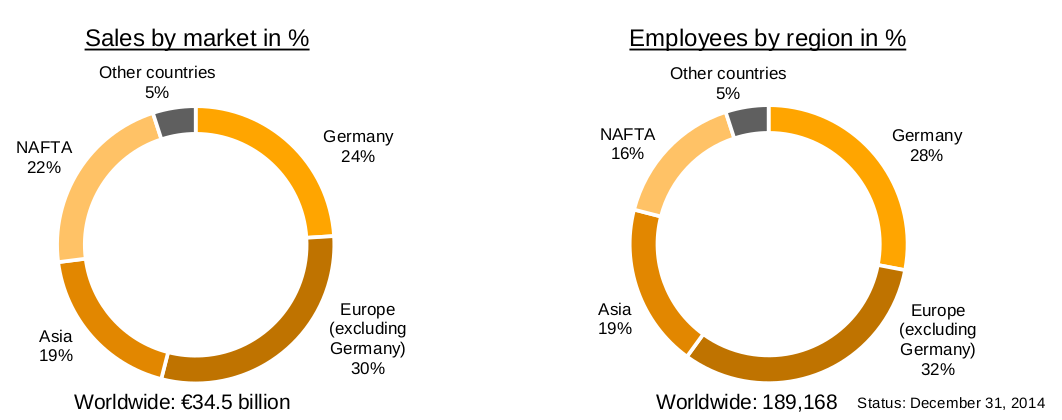
\includegraphics[width=17cm]{contents/images/caConti.png}
		 	\caption[Chiffre d'affaire et nombre d'employes (Annee 2014)]{Chiffre d'affaire et nombre d'employes (Annee 2014)\footnotemark{}}
		 	\label{fig:caConti}
		 \end{figure}
	 	\footnotetext{NAFTA : North American Free Trade Agreement}
		 En 2014, l'entreprise comptait plus de $189\;000$ employés dans le monde, comme le montre la figure \ref{fig:caConti} répartis dans 317 sites et 50 pays différents, dont la répartition est détaillée figure \ref{fig:repartitionConti}. Avec un chiffre d'affaire de 34.5 milliards d'euros au total, Continental est le numéro un du marché de production de pneus en Allemagne et est également un important équipementier automobile.

		 \begin{figure}[H]
		 	\centering
		 	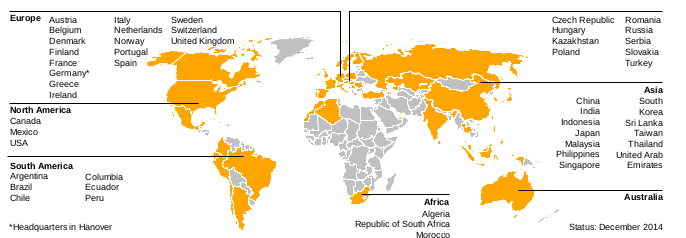
\includegraphics[width=18cm]{contents/images/repartitionConti.png}
		 	\caption{Répartition du groupe Continental dans le monde}
		 	\label{fig:repartitionConti}
		 \end{figure}		 

		\subsection{Histoire de l'entreprise}
		Continental est fondée en 1871 comme société anonyme sous le nom de <<\textit{Continental-Caoutchouc-und Gutta-Percha Compagnie}>> par neuf banquiers et industriels de Hanovre (Allemagne).

		Continental dépose l'emblème du cheval représenté sur la figure \ref{fig:logo}, comme marque de fabrique à l'Office impérial des brevets de Hanovre en octobre 1882. Ce logo est aujourd'hui encore protégé en tant que marque distinctive.
		\begin{figure}[H]
			\centering
			
\includegraphics[width=3cm]{contents/images/logoConti.png}
			\caption{Logo de Continental}
			\label{fig:logo}
		\end{figure}

		Le fabricant de pneus allemand débute son expansion à l'international en tant que sous-traitant automobile international en 1979, expansion qu'il n'a cessé de poursuivre depuis.
		
Entre 1979 et 1985, Continental procède à plusieurs rachats qui permettent son essor en Europe, celui des activités pneumatiques européennes de l'américain \textit{Uniroyal Inc.} et celui de l'autrichien \textit{Semperit}.

En 1995 est créée la division << \textit{Automotive Systems} >> pour intensifier les activités << systèmes >> de son industrie automobile.

La fin des années 1990 marque l'implantation de Continental en Amérique latine et en Europe de l'Est.

En 2001, pour renforcer sa position sur les marchés américain et asiatique, l'entreprise fait l'acquisition du spécialiste international de l'électronique \textit{Temic}, qui dispose de sites de production en Amérique et en Asie. La même année, la compagnie reprend la majorité des parts de deux entreprises japonaises productrices de composants d'actionnement des freins et de freins à disques. 

En 2004, le plus grand spécialiste mondial de la technologie du caoutchouc et des plastiques naît de la fusion entre \textit{Phoenix AG} et \textit{Conti'Tech}.

Enfin en juillet 2007, Continental réalise sa plus grosse opération en rachetant le fournisseur automobile \textit{Siemens VDO Automotive}. Ce rachat a permis à l'entreprise de multiplier son chiffre d'affaire par 2.5, passant ainsi de 13 milliards d'euros à plus de 34.5 milliards d'euros (chiffre de 2014).
		
		\subsection{Activités des différentes branches}
		\begin{figure}[H]
			\hspace{-55px}
			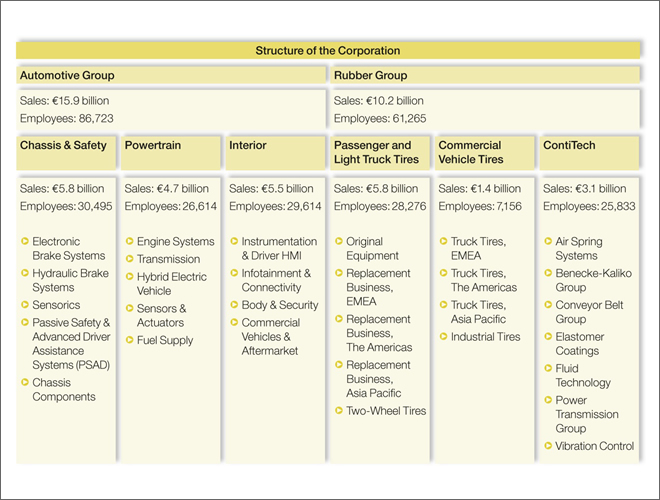
\includegraphics[width=21cm]{contents/images/structureConti.jpg}
			\caption{Structure de Continental}
			\label{fig:structConti}
		\end{figure}

		Comme on peut le voir sur la figure \ref{fig:structConti}, Continental est composée de cinq divisions. Ces dernières se chargent de développer et produire des équipements répondant aux besoins des clients. Pour cela elles sont composées de \textit{Business Units} qui ont chacune une activité bien particulière dans leur domaine de compétence. 

Durant mon stage, je travaillais au sein de \textit{P-ES} : 
\begin{description}
	\item[Division \textit{Powertrain}] S'occupe essentiellement du contrôle moteur, au niveau logiciel et matériel avec l'ECU\footnote{Engine Control Unit, Unité de calcul du contrôle moteur}
	\item[Business Unit \textit{Engine Systems}] Chargée de produire les équipements nécessaires au contrôle moteur tels que des calculateurs ou des injecteurs.
\end{description}

	\section{Le contexte de l'équipe TAS}
		J'ai travaillé dans l'équipe en charge des tests au niveau système ou logiciel dirigée par Corinne \bsc{Tarin}. Cette équipe doit aider à la vérification et la validation des programmes de contrôle moteur en fournissant des services de tests. 
		
 		\subsection{Le besoin} \label{besoinTests}
 		Le calculateur du contrôle moteur d'une voiture est un dispositif très important et à haut risque, en effet, une défaillance peut provoquer la mort de plusieurs personnes\footnote{Le programme d'une voiture comporte ainsi des fonctions dites << \textit{safety} >> tel que le régulateur, l'accélération, le freinage, \ldots}. Ainsi, le test est indispensable dans ce domaine, et doit être robuste. 

Le test des logiciel de contrôle moteur se fait aujourd'hui : 
\begin{itemize}
	\item << Soit à la main >> pour les tests d'intégration
	\item Soit à l'aide de scripts de test Python, écrit manuellement
\end{itemize}
Cependant, la taille des logiciels à tester est devenu particulièrement importante(Plusieurs milliers de variables, dans plus de 10 000 pages de spécifications\ldots). Cela appel à une automatisation plus forte des tests afin d'augmenter fortement la vitesse et la quantité de tests afin d'éliminer le maximum de bogue.

C'est dans ce contexte que l'équipe TAS intervient, c'est ainsi que je participe au développement d'un outil permettant d'automatiser des tests d'intégrations pour les équipes projet travaillant pour Ford.
 		\subsection{Les tests automatisés}

 		% P : Powertrain
 		% ES : Engine System
 		% SE :
 		% CV :
 		% TAS : Test & Automation Service
 		% TODO ajouter schéma de l'équipe dans Powertrain ?
 		
 		Pour ma part, j'opérais dans la partie test automatique. Cette << sous-équipe >> possède deux missions : 
 		\begin{itemize}
 			\item Le développement et l'exécution de scripts de tests de non-régression\footnote{Aussi appelés FaST : \textbf{F}unctions \textbf{a}nd \textbf{S}oftware \textbf{T}esting}. Ces scripts de tests s'exécutent sur bancs HiL\footnote{\textbf{H}ardware \textbf{I}n the \textbf{L}oop. Vous trouverez plus d'explications sur ce dispositif section \ref{wb}} avant la livraison des projets
 			\item Le développement et la maintenance d'outils logiciels notamment en utilisant la TA3 présenté section \ref{ta3}. Ceux-ci permettent d'améliorer la couverture et la qualité des tests. Ils doivent permettre aux développeurs de vérifier facilement et correctement leur travail, particulièrement pour des tests de non-régression bien que l'outil sur lequel je travail soit à destination de tests d'intégration.
 		\end{itemize}
	\subsection{Les outils de tests}
	Afin d'effectuer son travail, l'équipe TAS possède différents outils de tests. D'une part au niveau matériel avec des bancs de tests, mais aussi logiciel avec une plateforme écrite en Python.
	
		\subsubsection{Les bancs de tests}\label{wb}
		Afin de tester au mieux les programmes du contrôle moteur développés, ceux-ci sont d'abord testé via des simulateurs d'environnement véhicule. Ce simulateur permet de vérifier le programme avant d'effectuer des tests sur véhicule. Ces tests se font sur table dans un premier temps, pour deux raisons principales : 
		\begin{itemize}
			\item D'un part, les tables sont plus facilement accessible qu'un véhicule d'essais pour les équipes logicielles
			\item D'autre part, les tables possèdent plus de moyens afin d'observer finement l'ECU
		\end{itemize}
		
		Comme vous pouvez le voir figure \ref{fig:wb}, un banc de tests est composé d'un ordinateur, du calculateur appelé ECU pour \textit{\textbf{E}lectronic \textbf{C}ontrol \textbf{U}nit} et d'au moins deux équipements aidant aux tests. 
		
		Les deux équipements étant les suivants : 
		\begin{description}
			\item[Le HiL] Le \textit{\textbf{H}ardware \textbf{i}n the \textbf{L}oop} est un simulateur d'environnement véhicule. Ainsi l'ECU est branché sur le HiL et se comporte de la même manière que s'il était embarqué dans une voiture. Le HiL quant à lui est chargé d'envoyer les bons stimulus sur les pins de l'ECU, tel que l'injection, la vitesse de rotation du moteur, le starter \ldots
			\item[Debugger] Cet {appareil} est connecté au microcontrôleur de l'ECU via un port JTag. Il peut communiquer avec celui-ci afin d'effectuer différentes opérations. Tel que flasher le logiciel à tester, mettre des points d'arrêts sur le code, lire des variables, les modifier, changer des calibrations, \ldots
		\end{description}
	
		\begin{figure}[H]
			\centering
			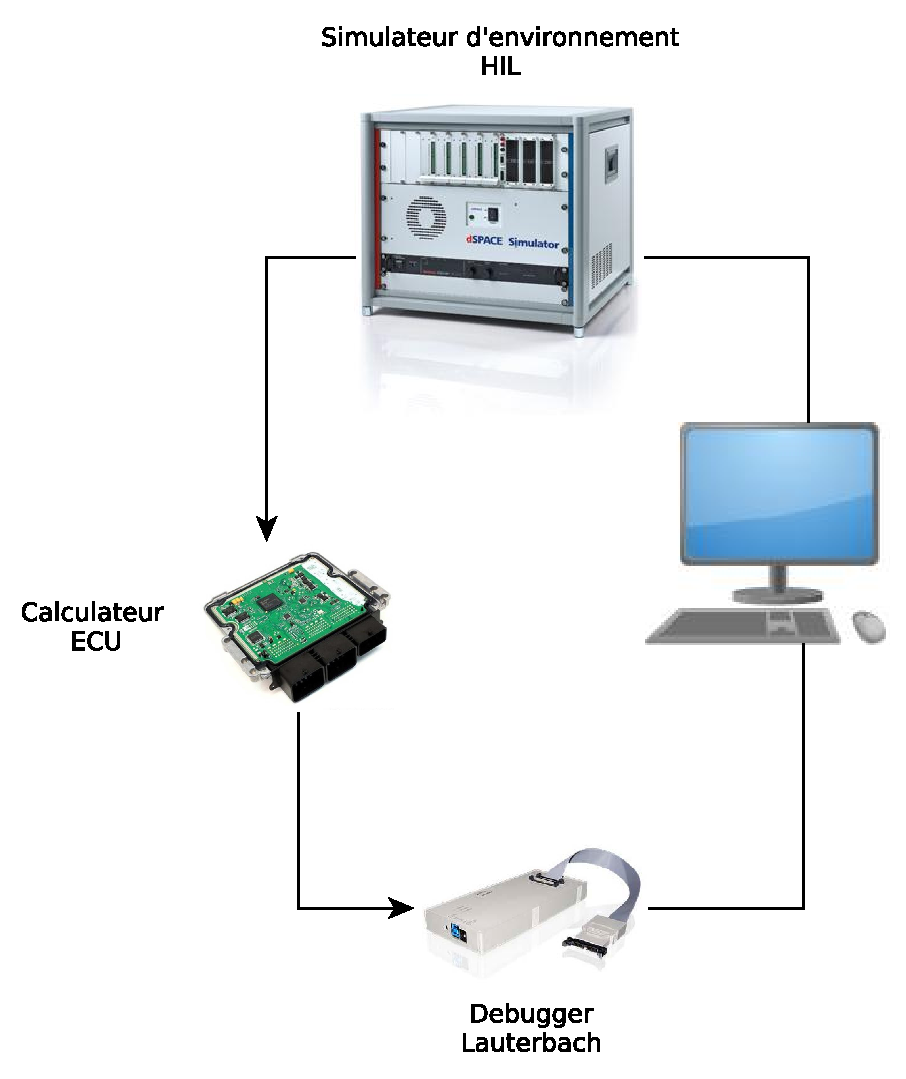
\includegraphics[width=12.1cm]{contents/images/WB.eps}
			\caption{Fonctionnement d'une table de tests : HIL DSpace, Debugger et ECU}
			\label{fig:wb}
		\end{figure}
				\begin{remarque}
					Un certain nombre d'équipes projet chez Continental utilise un troisième équipement qui n'est pas représenté ici, parce que notre plateforme ne s'en sert pas. Cet outil, nommé INCA, va interagir sur l'ECU via un bus CAN\footnote{Controller Area Network}.
				\end{remarque}
		Les différents équipements, ou \textit{device}, que nous pouvons voir sur cette figure sont ceux avec lesquelles notre nouvelle plateforme va communiquer afin d'effectuer des tests automatiques. 
		
			\subsubsection{La plateforme TA3}\label{ta3}
			\begin{wrapfigure}{l}{2.5cm}
				
\includegraphics[width=2.5cm]{contents/images/python.png}
			\end{wrapfigure}
			Actuellement, les équipes de tests disposent d'une plateforme appelée TA3. Celle-ci est une bibliothèque de classes écrites en Python. Jusqu'à présent, pour chaque objectif de test, il fallait écrire un script python utilisant la TA3. Ces scripts pilotent le banc HIL et le debugger afin d'envoyer des stimulis à l'unité de contrôle moteur et de vérifier que les réactions de celui-ci sont conforme aux spécifications de test.
			
			Cependant, cette plateforme pose un certain nombre de problèmes qui rend son utilisation difficile. D'une part, elle renvoie un trop grand pourcentage de faux-positifs\footnote{Lorsque l'on effectue des tests, le but du testeur est de trouver des bugs. Ainsi, un positif est l'apparition d'un bug, et donc un faux positif signifie que la plateforme montre des bugs, qui sont inexistants}, faisant perdre du temps au testeur. D'autres part, elle ne prend pas en compte certains besoins apparu récemment comme par exemple un système permettant de flasher automatiquement les ECU\footnote{Cela permettrai de scripter un test qu'on lancerai plus tard et de gagner du temps}, ou la possibilité de vérifier la fréquence de mise-à-jour de la production de variables\footnote{Ceci afin de contrôler le temps réel du calculateur}.
			
			Afin d'améliorer cette situation, l'équipe \textit{Tests \& Automation Service} développe une nouvelle plateforme.
			
%C'est dans ce contexte que l'équipe \textit{Tests \& Automation Service} intervient, elle doit fournir des outils aux développeurs afin de vérifier facilement et correctement leur travail, particulièrement pour des tests de non-régression, bien que l'outil sur lequel je travaille soit à destination de tests d'intégration.
 % ok
\setcounter{mtc}{3}
	\chapter{Le problème} \label{chapPb}
\begin{wrapfigure}{r}{0.60\textwidth}
\vspace{-25px}
\hspace{-30px}
\begin{minipage}{0.67\textwidth}
\minitoc
\end{minipage}
\end{wrapfigure}
Depuis longtemps, l'entreprise avait un problème afin d'effectuer des tests d'intégrations, notamment pour les projets à destination de Ford. Les tests demandaient du temps et de l'argent à l'équipe en charge de ces tests. Ainsi, deux ans avant mon stage de M1, une solution à été trouvée : le développement d'une nouvelle plateforme, \textit{GreenT}.

\vspace{-32px}
	\section{Les tests} \label{pbTests}
	Comme expliqué dans la section \ref{besoinTests}, le calculateur moteur est un système critique, il est donc indispensable de tester correctement celui-ci.

	\subsection{Le plugin}
	Dans le cadre de projets pour Ford, Continental ne développe pas l'intégralité du logiciel, en effet une partie est fournie par le client sous forme de << plugin >>. Le plugin est supposé correct, et ce n'est pas de notre ressort de le tester. Cependant, celui-ci va être interfacé avec les logiciels Continental : il est indispensable de vérifier que les deux parties fonctionnent ensemble lors de l'intégration.

	Pour cela, le client fourni un fichier appelé \texttt{Walkthrough}\footnote{Ce fichier est expliqué plus en détail section \ref{wt}} contenant la liste des variables du plugin avec toutes leur spécifications, ce fichier est au format \textit{Excel} : et il contient environ 900 variables différentes. Il est impensable de tester le fonctionnement d'autant de paramètres manuellement, ainsi l'équipe en charge de tester cette intégration effectue des tests de différence d'une version à l'autre : seules les variables ayant pu être impactées par une \textit{release} seront testées, il est supposé que les fonctionnement des variables restera inchangé.

	Trois problèmes se posent à cette méthode : 
	\begin{description}
		\item[La fiabilité des tests] Le test des seules différences ne permet pas nécessairement de détecter tous les problèmes (notamment avec des effets de bords…). De plus, une tâche répétitive peut entrainer des erreurs humaines.
		\item[Le temps de tests] Même en ne testant qu'une partie des variables, cela prend un temps considérable, il faut compter environ une semaine.
		\item[La disponibilité des bancs de tests]	Les tests s'effectuent sur des bancs de tests\footnote{Une photo d'un banc est disponible figure \ref{fig:photoHil}}, ces équipements permettent de simuler un environnement voiture autour du contrôleur moteur comme l'utilisation de la clé de démarrage, la tension de la batterie, la vitesse de rotation du moteur, ... Ces bancs sont peu nombreux dans l'entreprise, en raison de leur cout, leur disponibilité est compliquée. Il serait intéressant de pouvoir lancer des tests automatisés durant la nuit par exemple.
		
	\end{description}
	\begin{figure}[H]
		\centering
		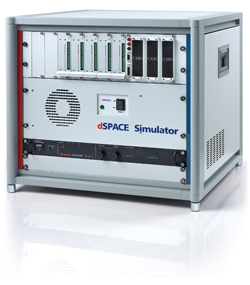
\includegraphics[width=7cm]{contents/images/hil.jpg}
		\caption{Exemple de banc de tests -- HIL DSpace}
		\label{fig:photoHil}
	\end{figure}

	\subsection{La plateforme TA3}
	Actuellement, les équipes de tests disposent d'une plateforme appelée TA3. Celle-ci est une bibliothèque de classes écrites en Python. Jusqu'à présent, pour chaque objectif de test, il fallait écrire un script python utilisant la TA3. Ces scripts pilotent le banc Hil et le l'outil de debug afin d'envoyer des stimulis à l'Unité de contrôle moteur(Noté ECU pour \textit{Electronic Control Unit}) et de vérifier que les réactions de celui-ci sont conforme aux spécifications de test.
	\begin{figure}[H]		
		\centering
		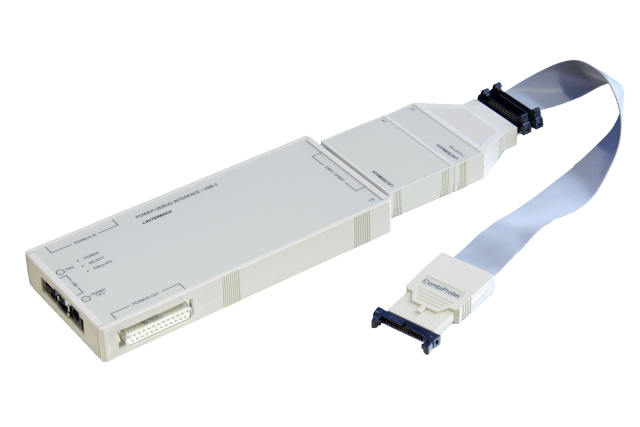
\includegraphics[width=7cm]{contents/images/trace32.png}
		\caption{Exemple de Debugger -- Trace32}
		\label{fig:photoHil}
	\end{figure}

	Cependant, cette plateforme pose un certain nombre de problèmes qui rend son utilisation difficile. D'une part, elle renvoie un trop grand pourcentage de faux-positifs, faisant perdre du temps au testeur. D'autres part, elle ne prend pas en compte certains besoins apparu récemments Comme par exemple un système permettant de flasher automatiquement les ECU, ou la possibilité de vérifier la fréquence de mise-à-jour de la production de variables.
\\~

	Afin d'améliorer cette situation, l'équipe Tests Automated Service développe une nouvelle plateforme.

	\section{La solution : \textit{GreenT}}
	Afin de résoudre les problèmes présentés dans la section \ref{pbTests}, une solution a été pensée en étudiant les besoins de l'équipe en charge des tests du plugin : le développement d'une plateforme de tests, appelé \textit{GreenT}.

	\subsection{Génération de tests automatiques}
	\subsubsection{Les tests d'intégration du plugin Ford}
	À court terme, cette solution devrait permettre de tester le plugin pour les projets Ford facilement et de façon efficace. Pour cela, les testeurs Continental vont ajouter des colonnes dans le document \texttt{walkthrough}, afin de spécifier la manière de tester les variables. La plateforme, sera capable d'analyser le document \texttt{walkthrough}, et de générer les tests automatiques. Le testeur n'aura plus qu'à lancer l'exécutable le soir, il reviendra le lendemain, tous les tests auront été exécutés avec un rapport détaillé pour chaque test.\\

	Ces tests s'effectueront sur des variables enregistrées lors de stimulation du contrôleur, afin de vérifier que celui-ci réagit de façon approprié.

	Cette plateforme permettra donc de tester facilement la dizaine de projets Ford, et une fois le test d'une variable spécifiée, il n'est plus nécessaire de le réécrire. À chaque nouvelle \textit{release} il suffira de relancer les tests : l'équipe n'aura à faire le travail qu'une fois, ensuite la réutilisation sera possible, les projets seront testés plus rapidement, plus efficacement, et plus souvent.

	\subsubsection{Les autres projets}
	À moyen terme, cette plateforme pourrait être utilisée pour les projets d'autres clients tel que Renault, afin d'effectuer là aussi des tests d'intégration, il était nécessaire de concevoir une plateforme qui puisse évoluer facilement, et avoir un fichier de spécifications en entrée qui soit légèrement différent d'un client à l'autre.

	En effet, les autres clients peuvent aussi fournir une partie du logiciel, avec un document de spécification des variables, celui-ci ne serait pas totalement identique, mais l'approche des tests s'en approchera.

	Il est également envisageable que la plateforme soit utilisée pour des tests d'intégration en interne, indépendamment des spécifications fournies par le client.

	\subsection{L'utilisation de \textit{GreenT} comme une bibliothèque}
		Une autre approche de notre plateforme, serait de s'en servir pour écrire facilemet des tests en Java, de façon plus efficace et plus robuste qu'avec la TA3 : notre plateforme doit donc également fonctionner comme une bibliothèque sans utilisation de générateur ou de parser, pour que le testeur puisse effectuer un test rapide. 

		Celui-ci apprendra à se servir de la plateforme, écrira en règle générale des tests assez courts et moins complexes que ceux que nous générerons, ceux-ci doivent être faciles à écrire.

	\subsection{L'exécution des tests}
	À long terme, l'objectif serait de pouvoir effectuer de l'intégration continue. 

	Il faut savoir que l'exécution de ces tests pourrait durer une quinzaine d'heures, en espérant qu'elle tienne sur une nuit. Cependant, il va arriver que les tests débordent et que lorsque le testeur revient, les tests ne soient pas terminés : le banc va être occupé alors que d'autres personnes en ont besoin, et le testeur n'a toujours pas les verdicts.

	 Nous souhaitons concevoir un système permettant l'exécution des tests sur des bancs en parallèle : on pourrait ainsi diviser le temps d'exécution par 2 ou 3, les tests tiendront sur une nuit et l'objectif principal serait tenu.

	 Mais le plus intéressant, serait d'utiliser le décalage horaire à notre avantage : lancer l'exécution des tests sur des bancs non utilisés dans d'autres pays, ainsi à toute heure de la journée il serait possible de lancer les tests. En effet, Continental étant présent dans la plupart des continents, il fait toujours nuit sur un site sur la planète. Après chaque étape d'intégration, on pourrait relancer les tests afin de vérifier qu'aucun bug n'a été introduit : le problème de la disponibilité des bancs serait alors résolu, et nous atteindrons une excellente sécurité.


	\setcounter{mtc}{4}
	\chapter{Organisation du développement}\label{chapOrganization}
\putminitoc \'Etant donné la complexité du projet et son importance, une organisation réfléchie est indispensable. Autant d'un point de vue humain, avec une gestion de projet et une gestion de l'équipe, que technique en utilisant certaines technologies nous aidant dans la tache.  Nous allons voir l'organisation qui a été mise en place afin d'être le plus efficace possible.

\section{L'équipe de développement}
Au cours de mon stage, trois développeurs travaillaient sur le projet \textit{GreenT} : Alain \bsc{Fernandez}, chef d’équipe et membre de
l’équipe \textit{Tests \& Automation Service}, Benjamin \bsc{Guerin}, apprenti, et moi-même, stagiaire au sein de la même équipe.

En tant que chef d’équipe, Alain \bsc{Fernandez} organisait les réunions et supervisait notre travail tout en corrigeant des bogues, et validait manuellement les rapports de tests\footnote{La validation manuelle des rapports est indispensable afin de vérifier que notre plateforme fournit des rapports fiables}. Benjamin \bsc{Guerin} se chargeait d'effectuer une étude de faisabilité sur l'amélioration visuelle des rapports de tests. Quant à moi je m'occupais de développer deux nouvelles fonctionnalités.\footnote{Cf chapitre \ref{collab}}.


À mon arrivée, la plateforme était quasiment opérationnelle, grâce à notre travail lors de mon précédent stage, et de l'avancement qui avait été fait durant cette année de césure. Je me suis donc d'abord renseigné sur les différentes améliorations et avancées du développement afin d'être rapidement opérationnel.  

Ensemble, nous avons convenu de documenter au maximum notre travail, afin de conserver une plateforme toujours à jour au niveau de sa documentation. Ainsi pour chaque modification, chacun de nous devait remplir un document de \textit{minutes d'étude}.

\section{La documentation : les \textit{minutes étude}}
Je suis arrivé en Mai sur un projet ayant été commencé 18 mois auparavant, ainsi beaucoup de choses existaient déjà : il était nécessaire de
garder l'existant. Afin de documenter notre travail, il a été décidé que pour chaque développement, que ça soit du bogue, de la fonctionnalité ou de la réorganisation du code, il était nécessaire de remplir un document Word.

Ce document comportait quatre grandes parties : 
\begin{description}
	\item[Analyse du besoin] Pourquoi ce développement est nécessaire, les cas d'utilisation pris en charge, ou non, les éventuelles discussions avec l'équipe cliente.
	\item[Analyse de l'existant] Retro-engineering permettant de comprendre le fonctionnement actuel du module que nous allons modifier, cette conception doit être statique, et dynamique, appuyé sur des schémas UML 2.
	\item[La solution] Conception de notre solution, ses limites, ses avantages. De la même manière que la partie précédente, la conception est statique et dynamique, avec des schémas UML 2.
	\item[Les tests] De quelle manière nous allons tester notre solution, aussi bien en tests unitaire qu'en tests d'intégration.
\end{description}

Ces différents documents pourront nous resservir plus tard pendant la maintenance, si un modèle doit être amélioré, ou comporte des problèmes, la relecture de la minute étude correspondante nous fera gagner beaucoup de temps.

\section{Outils de développement}
Afin de travailler de façon efficace, nous avons utilisés des outils aidant au développement. Ces outils ont été définis au début du projet, et n'ont pas évolués depuis.

\subsection{Java}
\begin{wrapfigure}{r}{3cm}
	
\includegraphics[width=2.5cm]{contents/images/logoJava.png}
\end{wrapfigure}
À mon arrivée, la partie client de notre plateforme était développée en Java dans sa version 6.0, Java nous permettant d'avoir un langage fortement typé, très puissant au niveau du paradigme Objet, connu de l'équipe, assez simple de déploiement et multiplateforme. 

Une de mes collaboration a été le passage à Java 8 nous permettant d'utiliser toute la puissance de Java, et d'avoir une plateforme qui soit à jour au niveau technologique.

\subsection{Git}
\begin{wrapfigure}{l}{3.5cm}
\vspace{-15px}
	
\includegraphics[width=2.5cm]{contents/images/logoGit.png}
\end{wrapfigure}
Nous avons utilisé \textit{Git} afin de faciliter le travail collaboratif d'une part, et de versionner le code du logiciel d'autres part. Git permet de fusionner les
modifications de plusieurs développeurs, tant que nous ne modifions pas le même fichier en même temps. Ainsi, la fusion de nos modifications était faite automatiquement. 

De plus, à chaque nouvelle modification, un << commit >>, permet de créer un point de restauration : il est alors possible de
récupérer n'importe quelle version du logiciel depuis son commencement. Nous y insérons un message clair expliquant ce qui a été fait, cela permet aux autres développeurs de l'équipe de se tenir au courant de l'avancement.

\subsection{Thrift et client-serveur}\label{thrift}
Notre plateforme fonctionne avec une architecture client-serveur, un client et deux serveurs. Le client écrit en Java, un serveur utilise
Python et le second est lui aussi en Java. Afin de faire communiquer les deux parties de notre application, nous avons utilisé \textit{Apache Thrift}. Il s'agit d'une bibliothèque ayant pour but les communications réseau inter-langage, dans le même principe que le protocole RMI\footnote{Remote Method Invocation}.

Ainsi, nous avons rédigé un fichier spécifiant les interfaces de notre serveur, c'est-à-dire les méthodes que nous souhaitions appeler en réseau. Une fois ce << contrat >> rédigé, il faut demander à Thrift de générer le code du serveur\footnote{Il est possible de demander la génération en C, C++, Python, Java, C\#, PHP, Ruby, \ldots}, et du client. Côté client, le service s'utilise directement, côté serveur, il faut implémenter une interface afin que notre service effectue les bonnes instructions. C'est donc le code généré qui va se charger de l'abstraction réseau.

\subsection{Eclipse}
\begin{wrapfigure}{r}{2.5cm}
	\vspace{-30px}
	
\includegraphics[width=2.5cm]{contents/images/logoEclipse.png}
\end{wrapfigure}
Nous développions tous sous le même environnement de développement Eclipse, avec le plugin \textit{Git} et le plugin \textit{PyDev}. Le
plugin Git permet d'avoir des outils aidant à la résolution d'éventuels conflits et le plugin PyDev permet de développer avec l'interpréteur
et la coloration syntaxique Python. 

\subsection{Antlr}
\begin{wrapfigure}{l}{2.5cm}
	
\includegraphics[width=2.5cm]{contents/images/antlr.jpg}
\end{wrapfigure}
Pour les besoins de notre plateforme, nous avons créé notre propre langage de test. Ce langage était assez riche, et la création d'un parser adéquate aurait pu être particulièrement long. Afin de nous faire gagner le maximum de temps, nous avons utilisé Antlr4.  \textit{Another Tool For Language Recognition} est un programme permettant de générer automatiquement un parser pour un langage donné. Ainsi, nous avions rédigés notre grammaire, Antlr quant à lui s'est chargé de nous générer un arbre de parcours syntaxique. À notre charge d'effectuer les bonnes actions durant le parcours de notre langage en spécialisant les classes générées par Antlr.
\newpage
\subsection{UML et \textit{Entreprise Architect}}
\begin{wrapfigure}{r}{3cm}
	
\includegraphics[width=2.5cm]{contents/images/logoEnterpriseArchitect.png}
\end{wrapfigure}
Nous avons travaillé avec la norme UML\footnote{Unified Modelling Language}~2 afin de concevoir la plateforme, en utilisant particulièrement des diagrammes de classes, mais aussi des diagrammes de cas d'utilisation ou d'activité. 

Pour dessiner ces diagrammes, et les noter dans la documentation, nous les pensions d'abord sur tableau blanc, mais ensuite nous avions besoin d'un outil puissant afin de les dessiner sur informatique. Pour cela nous avons utilisé \textit{Enterprise Architect}, un logiciel propriétaire permettant de créer tous les diagrammes de la norme UML~2.\\~

\subsection{SQLite}
\begin{wrapfigure}{l}{2.5cm}
	\vspace{-20px}
	
\includegraphics[width=2.5cm]{contents/images/sqlite.png}
\end{wrapfigure}
SQLite est un moteur de base de données relationnelle. Sa particularité est de ne pas reproduire le schéma habituel client-serveur mais d'être directement intégré aux programmes, la base de données étant stockée dans un simple fichier.

Nous nous en sommes servis afin de pouvoir stocker les différentes informations d'un test, ceci afin de pouvoir redémarrer une exécution grâce à cet état intermédiaire conservé en base de données.

\subsection{\LaTeX}
\begin{wrapfigure}{r}{2.5cm}
	
\includegraphics[width=2.5cm]{contents/images/logoLatex.png}
\end{wrapfigure}
Afin de rédiger ce rapport, et le diaporama de soutenance, j'ai utilisé \LaTeX{}, un langage et un système de composition de documents fonctionnant à l'aide de
macro-commandes. Son principal avantage est de privilégier le contenu à la mise en forme, celle-ci étant réalisée automatiquement par le système une fois un style défini. 
	
	\setcounter{mtc}{5}
	\chapter{\textit{GreenT} : fonctionnement général}\label{chapGreent}
\putminitoc

Comme nous l'avons montré dans le chapitre \ref{chapPb}, l'entreprise a besoin d'un nouvel outil aidant aux tests d'intégration : \textit{GreenT}. 

Nous allons donc voir le développement et la conception de cette plateforme de tests.

Au début de mon stage, le projet ayant un an, les fonctionnalités développées ci-dessous étaient déjà faites. Je suis cependant intervenu
sur la plupart d'entre elles soit pour des corrections de bogues d'une part, soit à des fin d'améliorations d'autre parts.

Avant de présenter mon travail, que vous trouverez chapitre \ref{collab}, il est nécessaire de présenter le fonctionnement général de
cette plateforme afin d'en avoir une vue d'ensemble.

\section{Le fichier Walkthrough}\label{wt}
Le fichier \textit{Walkthrough} est un fichier qui sera fourni par la personne en charge des tests, c'est un fichier au format Excel qui contient les informations
de chacune des variables à tester. Il contient ainsi un très grand nombre de colonnes, bien que seule une partie de celles-ci nous
intéressent. Certaines colonnes ont été remplies par le fournisseur du plugin, d'autres colonnes sont ajoutées dans le seul but de la
génération de tests automatiques par \textit{GreenT}. Voici les informations les plus intéressantes : 

\begin{description} 
	\item[Nom de la variable] Le nom de la variable testée : il existe un nom court et un nom long.
	\item[Informations aidant à la conversion des données] Certains équipements\footnote{Vous trouverez plus d'informations sur le fonctionnement d'une table de tests section \ref{wb}}, à l'instar du \textit{debugger} ne fonctionnent qu'avec des
	valeurs Hexadécimales. À la charge de \textit{GreenT} de convertir ces données vers des valeurs physiques exploitables par
	le testeur. Ces colonnes contiennent les informations nécessaires au calcul de conversion\footnote{Informations tel que le
		domaine de définition physique et le domaine de définition hexadécimal, avec ces deux informations il est possible d'effectuer les conversions physique vers hexadécimal}.
	\item[Nécessité d'un test automatique] Un \texttt{GreenTTest} ne sera généré que si la colonne vaut \textit{Yes}.
	\item[Statut du test] La plateforme éditera automatiquement cette colonne afin de reporter le statut du test\footnote{Un test pouvant être \textit{Green} ou \textit{Red}
		mais peut aussi comporter une erreur, tel qu'un problème d'exécution ou de génération, \ldots}.
	\item[Précondition (cf section \ref{stim})] Contient un scénario d'initialisation du \textit{workbench} : tension de départ,
	démarrage de l'ECU, \ldots
	\item[Scénario de stimulation (cf section \ref{stim})] Contient un ou plusieurs scenarii de stimulation destinés à faire générer au HiL un certain nombre de stimuli.
	\item[\texttt{ExpectedBehavior} (cf section \ref{expectedBehavior})] Contient une expression évaluant les variables ayant été enregistrées durant la stimulation : \textit{GreenT} devra vérifier que cette expression est correcte à tout instant de la stimulation.
	\item[Variable à enregistrer (cf section \ref{expectedBehavior})] Contient les variables devant être enregistrées durant un
	scénario, en plus des variables présentes dans l'\textit{expected behavior}. Celles-ci peuvent servir en tant que données
	contextuelles permettant de mieux cerner le résultat d'un test.
	\item[Informations du test (cf section \ref{report})] Plusieurs colonnes telles que la sévérité, le responsable du test, des commentaires, \ldots
\end{description}


\begin{figure}[H]
	% TODO CHange WT version
	\hspace{-35px}
	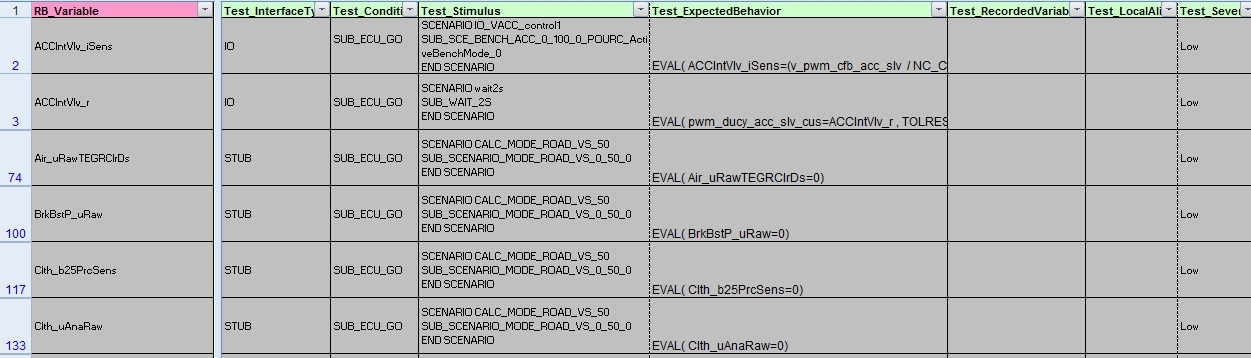
\includegraphics[width=20cm]{contents/images/walkthrough.png}
	\caption{Aperçu d'un fichier Walkthrough}
\end{figure}

\section{Fonctionnement Global}
Le développement de \textit{GreenT} inclut un certain nombre de fonctionnalités attendues par le client et indispensable à son fonctionnement. D'autres fonctionnalités pourront apparaître plus tard en fonction des besoins.

Les principaux modules sont les suivants, avec leurs interactions schématisées figure \ref{fig:generalDiag} : 
dans des objets ovales sont représentés des fichiers, les carrés représentent des modules de la plateforme et les flèches en pointillés un transfert réseau, les couleurs représentent les différents modules de la plateforme.

\begin{figure}[H]
	\hspace{-25px}
	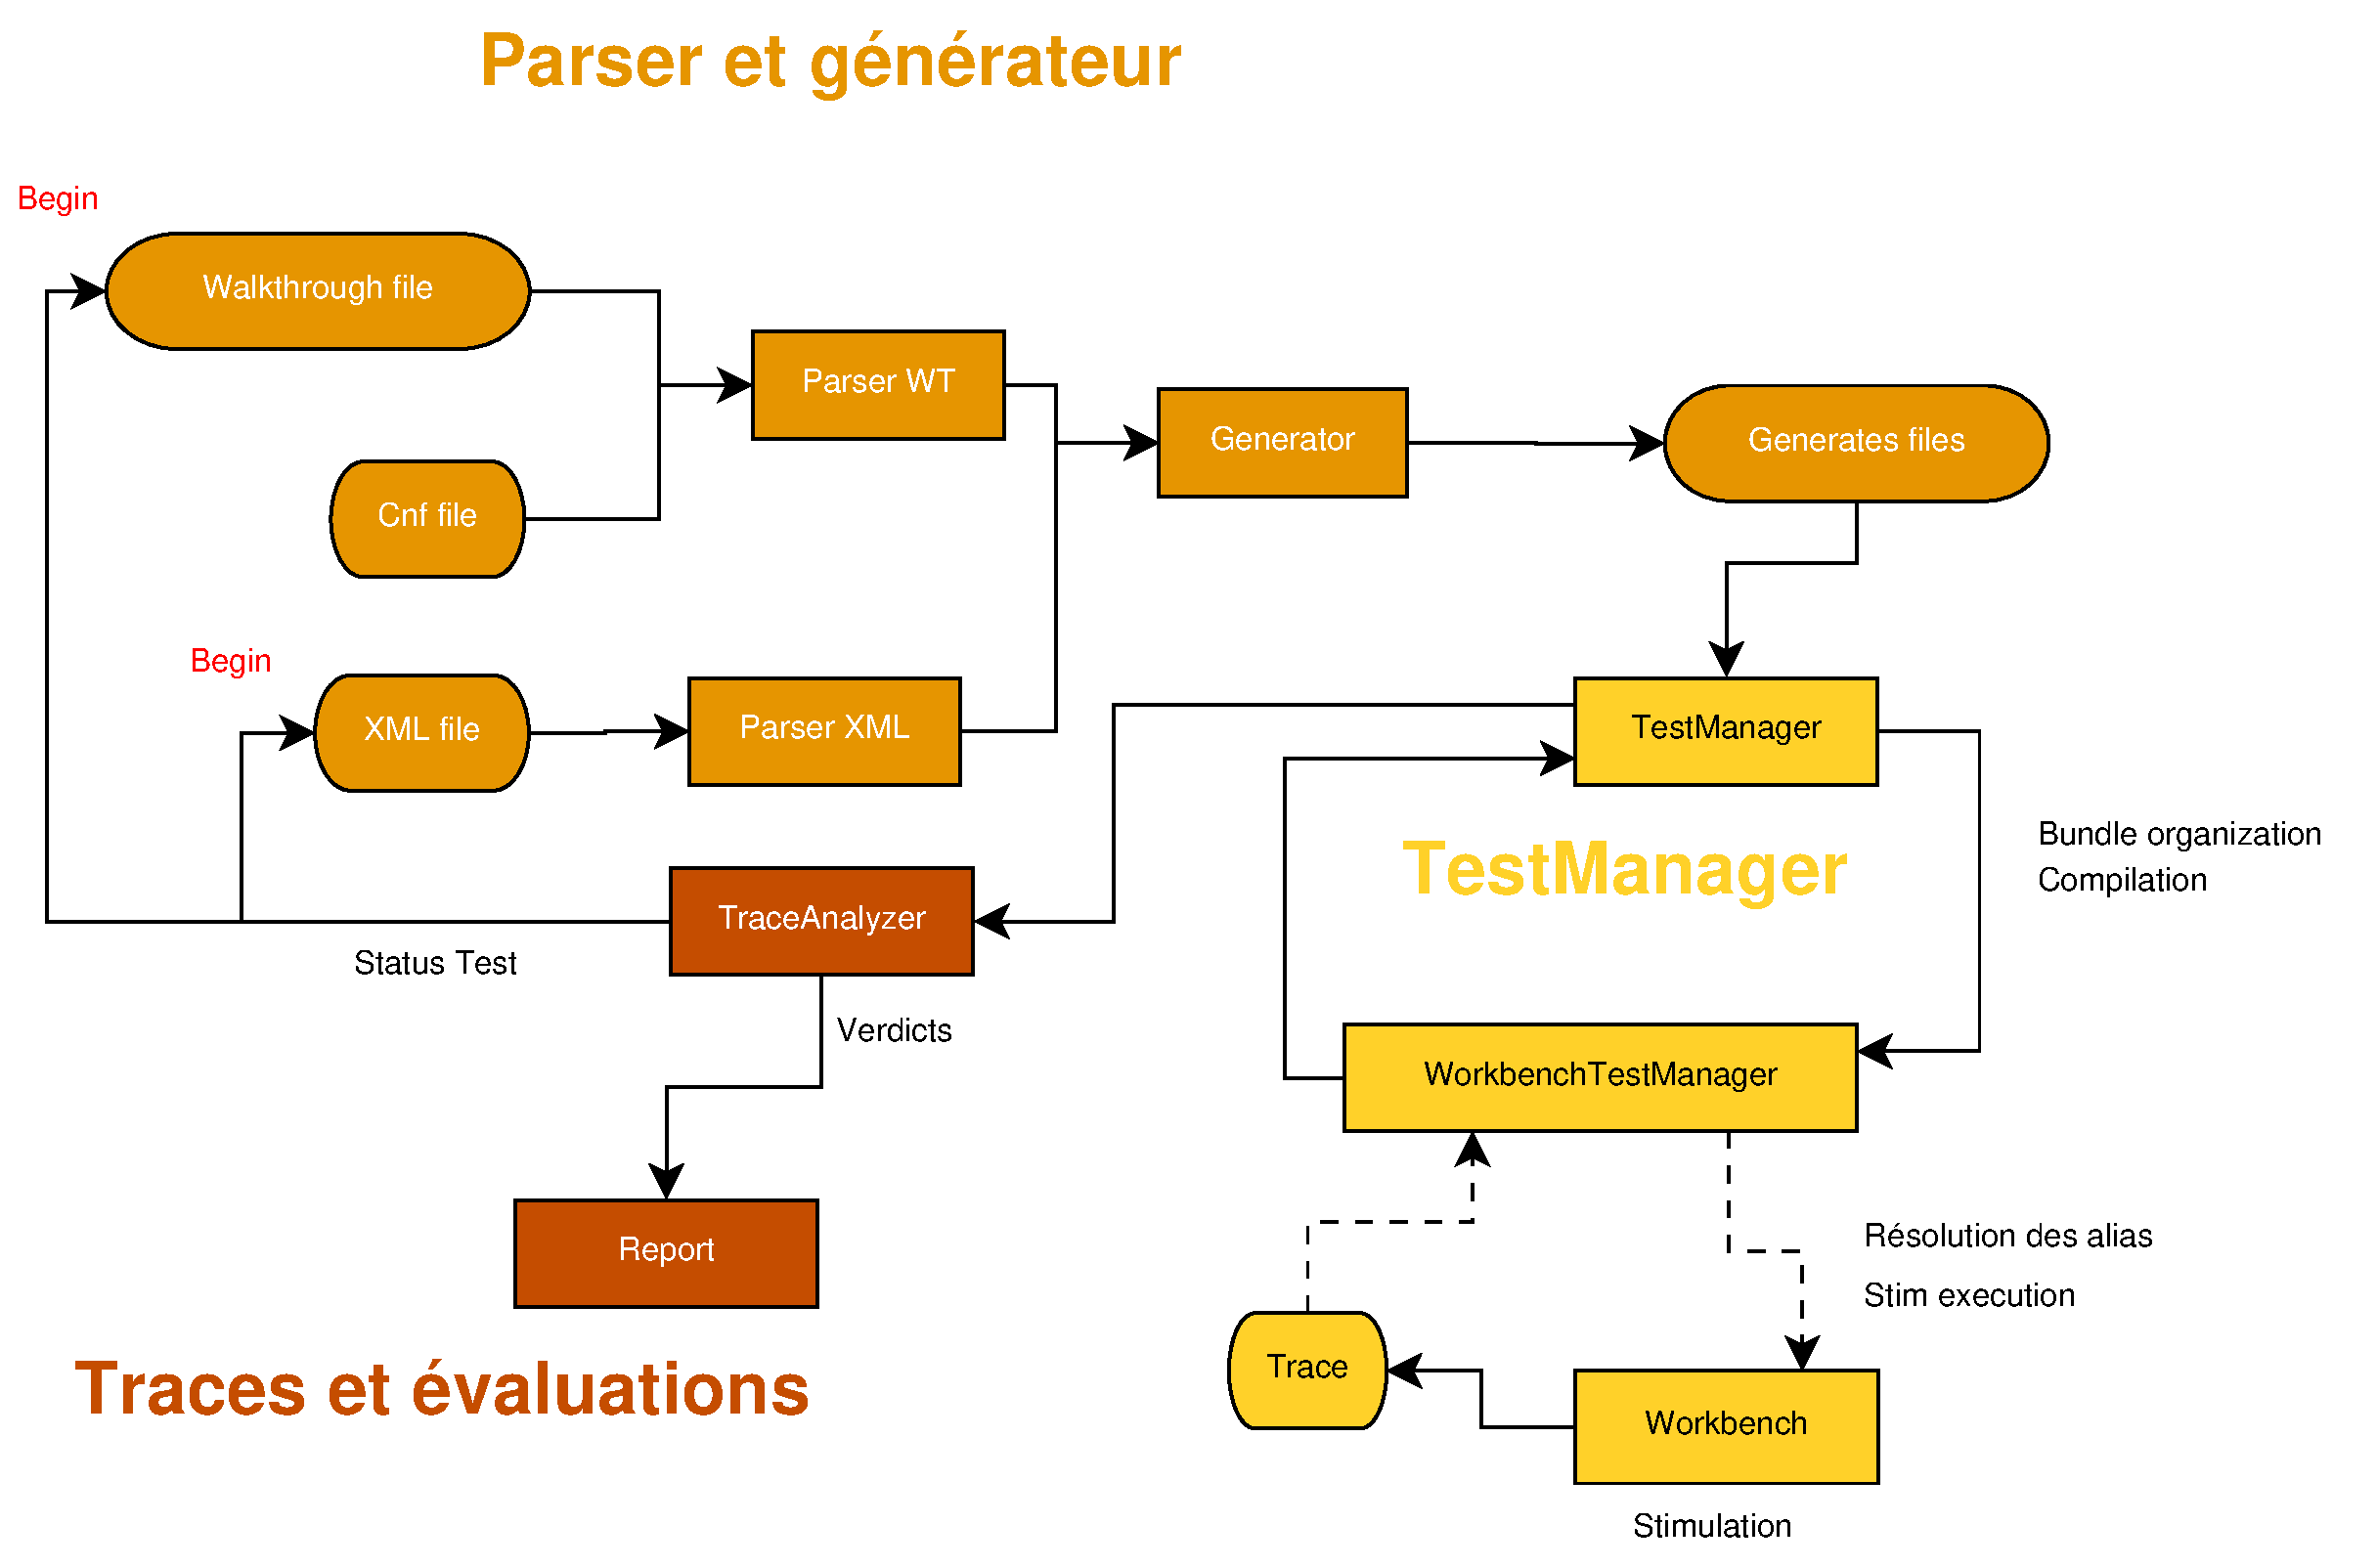
\includegraphics[width=20cm]{contents/images/generalDiag.eps}
	\caption{Fonctionnement général de la plateforme \textit{GreenT}}
	\label{fig:generalDiag}
\end{figure}	

Dans la figure \ref{fig:generalDiag}, vous pouvez voir des flèches en pointillés représentant des échanges réseau. En effet
l'exécution des stimulations et l'enregistrement des traces se fait par un contrôle distant des bancs de tests\footnote{La
	schématisation du fonctionnement d'un banc est disponible section \ref{wb} figure \ref{fig:wb}}.

Les principales fonctionnalités demandées par le client sont disponibles sur le client, la majorité peuvent s'effectuer en local : 
\begin{itemize}
	\item Le parsing et la génération (section \ref{generation})
	\item L'organisation en Bundle afin d'optimiser le temps d'exécution des tests (section \ref{testManager})
	\item La production de rapports détaillés (section \ref{expectedBehavior})
\end{itemize}~\newline
Alors que d'autres fonctionnalités vont nécessiter la présence de serveurs et de connexion réseau permettant d'effectuer ces actions
: 
\begin{itemize}
	\item Les stimulations (section \ref{stim})
	\item Les enregistrements des traces (section \ref{stim})
\end{itemize}
\vspace{-10px}
\section{Les fonctionnalités du Client}
Afin de répondre au mieux aux attentes du client, il a été choisi d'utiliser le langage Java pour développer notre client, ceci en raison de
divers avantages comme le côté multi-plateforme, son typage fort et sa forte communauté qui permet ainsi une maintenance facilitée. 

\subsection{\textit{Parsing} et Génération}\label{generation}
Le but premier de la plateforme est d'effectuer des tests automatiques, il est ainsi indispensable d'avoir un système d'automatisation, au travers d'une génération.

Pour cela, nous avons un parser : il analyse un certain type de fichier\footnote{Nous ne commencerons qu'avec le \textit{Walkthrough} pour débuter, mais dans le futur nous pourrions avoir des fichiers XML, des bases de données, \ldots} et en retire pour chaque test, le scénario de précondition, les différents scénarii de stimulations, leur \textit{Expected Behavior}, les données qui devront être enregistrées ainsi que différentes informations sur le test\footnote{Responsable du test, sévérité, commentaires, nom de la variable, \ldots}.

Une fois toutes ces données acquises, il les transmet à un générateur qui est en charge d'écrire les fichiers Java de chaque test, tous sont organisés dans un dossier temporaire avec un dossier par test. Le \texttt{TestManager} peut ensuite traiter ces données.

\begin{exemple}
Le testeur souhaite vérifier le bon fonctionnement des ventilateurs de refroidissement du moteur. Ci-dessous les différentes cellules qui pourraient être renseignées par le testeur pour ce cas de test. Nous verrons ce qu'effectuent précisément ces actions dans la suite de la section.	

\begin{tabular}{p{4cm}|p{6.5cm}|p{5.4cm}}
	\textbf{Précondition} & \textbf{Scénario de Stimulation} & \textbf{Expected Behavior}\\
	\hline
	\begin{minipage}{0.1\linewidth}
		\begin{lstlisting}[framerule=0pt,language=gtl]
// Tension batterie
HIL_VB = 13;
// Clé moteur
HIL_KEY = 1;
// Vérifications
CHECK(HIL_KEY = 1 
	&& HIL_VB = 13);
	\end{lstlisting}
	\end{minipage} & 
	\begin{minipage}{0.1\linewidth}
		\begin{lstlisting}[framerule=0pt,language=gtl]
// Rampe de vitesse véhicule
// de 0 à 50km/h par pas de 1 
// toutes les secondes	
RAMP(HIL_VS, 0, 50, 1, 1);
		\end{lstlisting}
	\end{minipage} 
	&
		\begin{minipage}{0.1\linewidth}
			\begin{lstlisting}[language=ada,framerule=0pt,language=gtl]	
if temperature > max then
 // Ventilateur allumé
 EVAL(ventilateur_on = 1); 
else
 // Ventilateur éteint
 EVAL(ventilateur_on = 0); 
end if
			\end{lstlisting}
		\end{minipage} 
	\\
\end{tabular}
\end{exemple}

\subsection{Stimulation} \label{stim}
\vspace{-20px}
Afin de tester une variable du plugin, les développeurs vont utiliser des alias présents sur un device : actuellement, un HiL ou un debugger, prochainement nous pourrions en utiliser d'autres. Ces alias permettent de simplifier le travail du spécifieur, il n'aura pas à retenir une adresse d'un élément sur le HiL, un simple alias permet de lui faire cette abstraction et ce raccourci.

Le spécifieur va rédiger des scénarii de stimulation, ceci afin de mettre le contrôleur dans certaines conditions. Son but sera ensuite de vérifier que ces variables restent cohérentes vis-à-vis du scénario effectué. 

Un scénario particulier doit être spécifié : une précondition qui a pour but d'initialiser les équipements et certains alias afin d'avoir un état de stimulation qui soit cohérent et identique à chaque lancement du scénario. Ce scénario sera effectué avant le lancement de chacun des scénarii de stimulation.

Durant l'exécution d'une stimulation, les variables nécessaires sont enregistrées afin de pouvoir produire des rapports et des
verdicts ensuite.
\begin{exemple}
	Comme nous l'avons vu section \ref{generation}, le testeur nous a donné un scénario de stimulation ainsi qu'un scénario de précondition. Le code généré va ainsi communiquer avec le serveur HiL afin qu'il envoie les bons stimuli à l'ECU.

	Comme mis en commentaires, le scénario de précondition va mettre la batterie à 13 Volts, et mettre la clé, nous allons ensuite vérifier que cette action a bien été faite. Si tel est le cas, le scénario de stimulation va être effectué. Celui-ci va appliquer une rampe de vitesse, notre véhicule va aller de zéro à cinquante kilomètre-heure avant de retourner à l'arrêt.	
\end{exemple}

\subsection{Les traces et leurs évaluations}\label{expectedBehavior}
Lorsqu'un scénario de stimulation s'exécute, un certain nombre de variables sont enregistrées : ces variables sont stockées sous la forme d'une trace au format CSV\footnote{Comma Separated Values}, qui pourra plus tard être représentée sous forme de courbe. 

Une fois que la trace est complète, il est nécessaire de l'évaluer : le spécifieur a décrit le comportement attendu dans la colonne \textit{Expected Behavior} détaillant dans quel cas le test est correct. Cette expression va être transformée en arbre logique afin de l'évaluer à tout instant de la trace. 

\begin{exemple}
	Durant notre rampe véhicule, le \textit{debugger} a enregistré différentes variables, en l'occurence nous avons enregistré les trois variables présentes dans notre \textit{Expected Behavior} : la température	du moteur -- \texttt{temperature}, la température maximum sans ventilateur -- \texttt{max}, ainsi que l'état de notre ventilateur -- \texttt{ventilateur\_on}.
	
	Ces variables ont été enregistrées durant l'intégralité de la rampe véhicule qui à eu une durée de cinquante secondes. À la fin de la stimulation, le serveur retourne ainsi une trace de cinquante secondes contenant toutes les variables. \textit{GreenT} peut ensuite évaluer notre \textit{expected behavior} sur l'intégralité de l'enregistrement.
\end{exemple}
\subsection{Le module TestManager}\label{testManager}
Comme le montre la figure \ref{fig:generalDiag}, la classe \texttt{TestManager} est le chef d'orchestre de \textit{GreenT}, il a donc un certain nombre de responsabilités. 

Il va d'abord organiser les différents tests en un concept que nous avons appelé \textit{Bundle}, ceci dans un but d'optimisation du temps d'exécution. En effet, si nous avons 1000 tests de 2 minutes, cela ferait plus de trente heures d'exécution. Pour palier à ce problème, nous avons deux stratégies :
\begin{itemize}
	\item Le regroupement de tests ensemble, si deux tests possèdent le même scénario de stimulation, alors nous n'executerons qu'une seule fois ce scénario, et évaluerons la trace pour chacun des tests. Ce regroupement est appelé <<Bundle>>.
	\item Même avec notre stratégie des Bundles, l'exécution pourrait être encore trop longue. Ainsi, il est possible d'utiliser plusieurs tables en simultané. Le temps d'exécution est ainsi divisé par le nombre de tables. 
\end{itemize}

Afin d'être le plus souple possible, il existe plusieurs modes d'exécution de la classe \texttt{TestManager} : 
\begin{description}
	\item[Check only] Essaye de parser les différents fichiers, et vérifie que ceux-ci ne comportent aucune erreur de grammaire, d'alias introuvable, d'écriture sur un alias en lecture seule etc... Cela permet à l'auteur des cas de test de se vérifier sans avoir besoin de table de test.
	\item[Parse and generate bundles] Parse les fichiers et génère des jars exécutables répartis en bundle
	\item[Parse and execute] Parse les fichiers, génère les jars pour les bundles et les exécute : c'est le mode << classique >>.
	\item[Restart test execution] Redémarre une exécution qui se serait mal terminée. Ceci à l'aide d'une base de données SQLite. Cette base de données contient toutes les informations des différents scénarii et sera capable de redémarrer à l'endroit où une coupure à eu lieu. Cela évite de devoir effectuer de nouveau trente heures d'exécutions si le problème à eu lieu sur la fin.
\end{description}

\subsection{Production de rapport détaillé}\label{report}
La plateforme a en charge la production d'un rapport détaillé pour chaque test. Ce rapport contiendra un certain nombre d'informations, et permettra au testeur de comprendre pourquoi le test n'est pas passé. Voici les informations que contiendra ce rapport : 

\begin{itemize}
	\item Nom du test, de la variable à tester
	\item Nom du responsable du test
	\item Sévérité du test
	\item Pourcentage de branches de l'\textit{Expected Behavior} renvoyant faux(Test << Rouge >>), n'ayant pas pu être testé(Test << Gris >>) et étant correct(Test Vert)
	\item Le testeur aura à sa disposition les expressions concernées par un résultat Rouge ou Gris.
	\item Les colonnes utiles du \textit{Walkthrough}
\end{itemize}

Actuellement, les rapports se font au format Excel avec l'intégralité de notre enregistrement et pour chaque instant d'enregistrement(timestamp), un verdict. Un
exemple de rapport est accessible en Annexe \ref{apendixReport} page \pageref{apendixReport}. 

Dans un futur proche, ces rapports pourraient être générés dans un format Web avec une possibilité de naviguer entre plusieurs tests, et
d'avoir un affichage des courbes de manière graphique.

\subsection{Mise à jour du Walkthrough}
Une fois l'analyse d'un test exécuté, un verdict global est mis dans le fichier \textit{Walthrought} : ce verdict est consolidé en fonction des rapports détaillés. Ainsi, un test sera vert si l'expression a été validée sur l'ensemble de la trace, le test sera rouge dans le cas contraire.

\begin{remarque}
	En cas d'erreur à la génération\footnote{Mauvaise syntaxe, variables inexistantes, \ldots} ou à l'exécution\footnote{Problèmes réseaux, variable non trouvée, communication entre l'ECU et le debugger, \ldots}, la plateforme doit afficher un message d'erreur clair au niveau du test afin que l'utilisateur soit conscient du problème. Libre à lui de corriger le test si nécessaire, ou de le signaler si cela semble être un bogue. Ce message d'erreur est reporté automatiquement dans le \textit{Walkthrough}.
\end{remarque}

\section{Les fonctionnalités des serveurs}\label{wbgt}
Comme expliqué précédemment, \textit{GreenT} va avoir en charge l'exécution de stimulations. Celles-ci vont communiquer avec une table de
test. Actuellement une table est composée de deux équipements différents, comportant chacun leur serveur : 
\begin{itemize}
	\item Un HiL, Hardware In the Loop, simulateur d'environnement véhicule
	\item Un Debugger permettant de voir l'état du programme présent dans l'ECU
\end{itemize}

\begin{figure}[H]
	\centering
	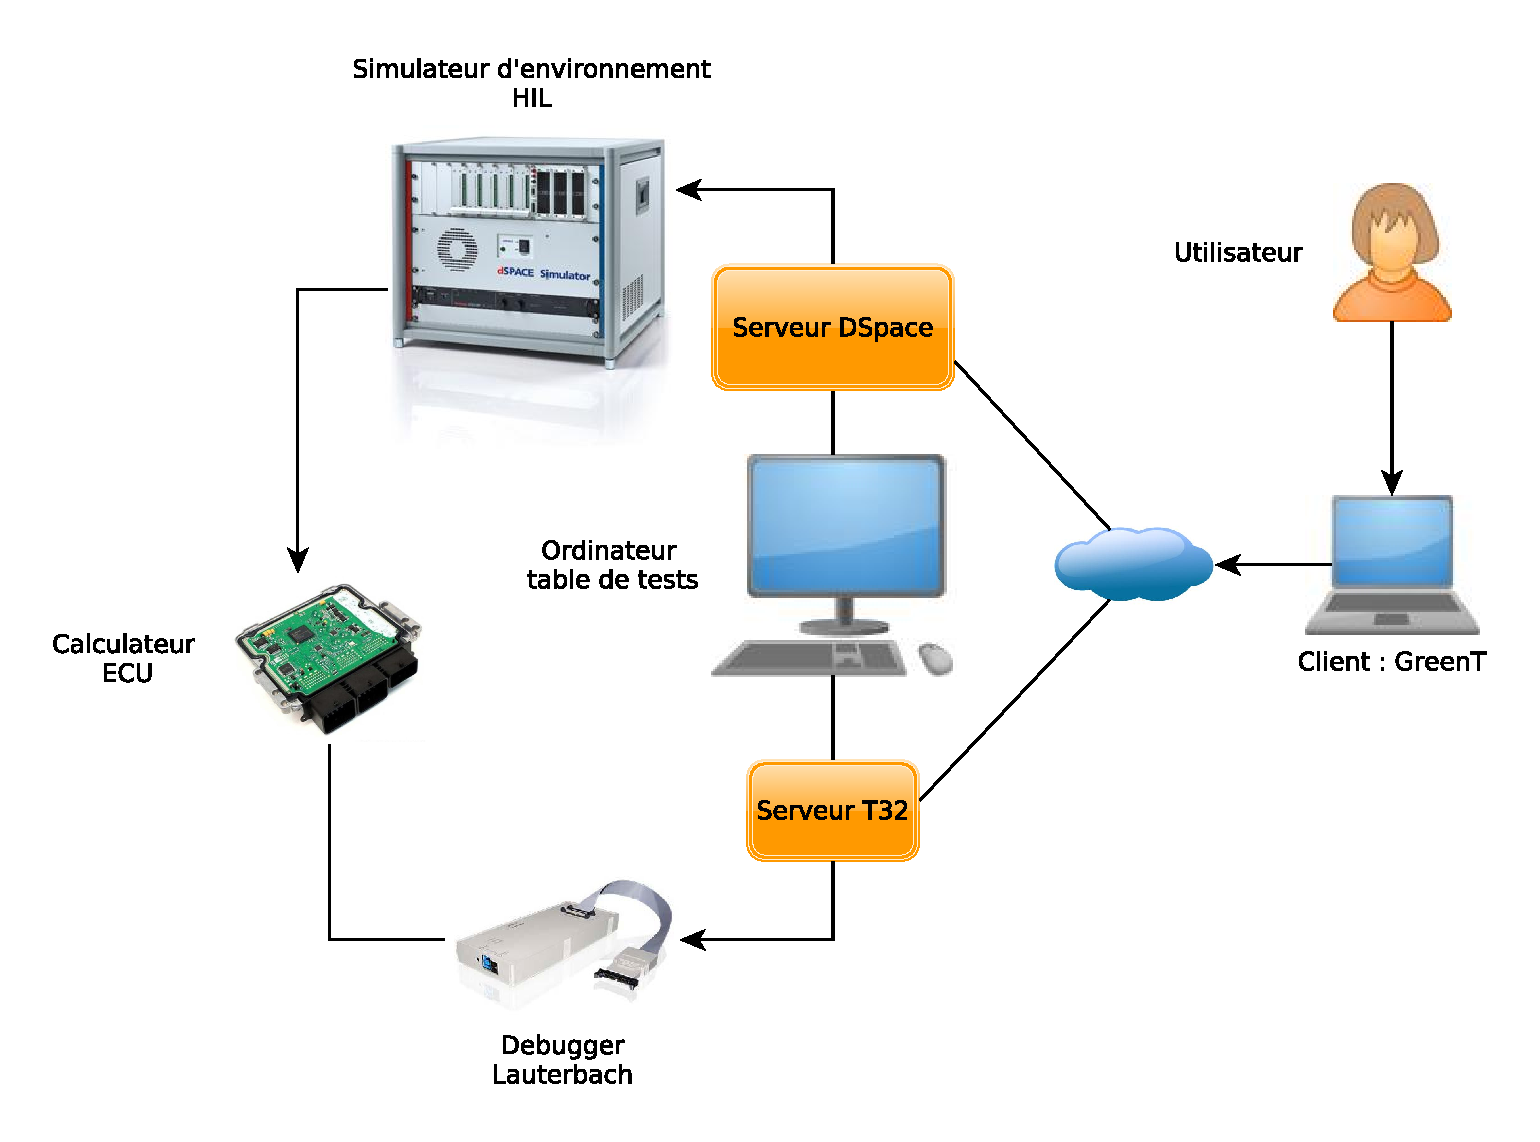
\includegraphics[width=17cm]{contents/images/network.eps}
	\caption{Communications de la plateforme}
	\label{fig:wbgt}
\end{figure}

Au début du développement de la plateforme, il a été décidé que les serveurs devront être le plus simple possible pour plusieurs raisons
: 
\begin{itemize}
	\item Donner accès à un maximum de fonctionnalités en mode << offline >>, c'est-à-dire sans accès à une table de test
	\item Rabattre le maximum de fonctions métier près du client pour centraliser au maximum le fonctionnement et éviter la maintenance superflue
	\item Avoir la possibilité de réutiliser les serveurs pour d'autres projets
	\item Pouvoir ajouter facilement un nouveau \textit{device}, qui ne nécessiterai que l'ajout d'un nouveau serveur relativement simple
\end{itemize}

\subsection{Le serveur Debugger, contrôle de Trace32}\label{T32server}
Le serveur Debugger propose des services basiques permettant de répondre aux besoins :
\begin{itemize}
	\item Flasher le logiciel dans la flash de l'ECU
	\item Démarrer l'ECU
	\item Arrêter l'ECU
	\item Lire une variable ou une calibration
	\item Modifier une variable
	\item Enregistrer des variables
\end{itemize}~

\begin{wrapfigure}{l}{3cm}
	\vspace{-40px}
	
\includegraphics[width=2.5cm]{contents/images/logoJava.png}
\end{wrapfigure}
Afin d'effectuer ces actions, le serveur s'appuie sur une API fournie par l'outil Trace32 permettant de contrôler le debugger. Ainsi tous nos services vont s'appuyer sur cette API. C'est pour cette raison que ce serveur est développé en Java afin de pouvoir utiliser
facilement ces fonctions.

\subsection{Le serveur HiL, contrôle du ControlDesk DSPace}
Le HiL contient une base de données, représentant un modèle simulant l'environnement véhicule. Ce modèle à pour but de se rapprocher au maximum du fonctionnement réel de notre moteur.

Le serveur DSpace va devoir lui aussi répondre aux différentes stimulations, ainsi ces services sont relativement similaire : 
\begin{itemize}
	\item Modifier une valeur du modèle
	\item Lire une valeur du modèle
	\item Enregistrer des valeurs
\end{itemize}~

\begin{wrapfigure}{r}{3cm}
	
\includegraphics[width=2.5cm]{contents/images/python.png}
\end{wrapfigure}
Ce serveur a été développé en réutilisant une partie de ce qui avait été fait pour la TA3, présenté section \ref{ta3} afin de ne pas
<< réinventer la roue >>. 

À l'instar du serveur Debugger, nous utilisons une API fournie par l'outil permettant de contrôler le HIL : ControlDesk. 
C'est ainsi que ce serveur est développé en Python afin de répondre à cette contrainte : l'API du ControlDesk est en Python. Ainsi, l'utilisation de Thrift, permettant de faire dialoguer du Java côté client et du Python côté serveur facilement, nous aura particulièrement aidé.



	\setcounter{mtc}{6}
	\chapter{Ma collaboration au projet}\label{collab}
\putminitoc
Après avoir défini plus en détails les besoins de notre outil et son fonctionnement général, nous allons maintenant voir en détail de quelle manière j'ai contribué à ce projet. Le développement s'est effectué en deux grandes étapes. D'une part, la finalisation de la première version via la production de rapports détaillés, et ce jusqu'en Janvier. Suivi par des améliorations afin que l'outil puisse être utilisé par le plus grand nombre, notamment la généralisation de l'outil aux projets Renault. 

\section{La difficulté de productions de rapports}
Au début du développement de l'outil, une solution d'analyse avait été mise en place, cependant cette solution ne pouvait fonctionner comme nous allons le voir. C'est ainsi que nous avons développé un autre algorithme de production de verdicts, basé sur les récurrence de calculs et un concept d'entrée et de sortie de calculs. 

\subsection{Les calculs du logiciel}
	Un logiciel embarqué temps réel effectue différents tâches de calculs à des récurrences fixes. C'est-à-dire que chaque tâche doit être deterministe et s'exécuter au bout d'un temps donné, moyennant une petite marge d'erreur. Dans les logiciels que nous testons, ces tâches peuvent être exécutés toutes les dix milisecondes par exemple. 
	
	% TODO Super task

	Comme le montre la figure \ref{fig:task}, une tâche de calcul prends des donnés en entrée, et écrit un résultat dans une ou plusieurs variables de sortie. Dans le cadre de l'intégration du plugin, un certain nombre de tâche ont pour but la connection de ce plugin. Ainsi, elles vont prendre les des données du plugin en entrée, et écrire le résultat dans une variable de chez Continental. 

\subsection{Le problème de l'existant}
% TODO capture d'écran ancien rapport foiré
En début du projet, il avait été décidé que nous allions évaluer une trace à l'ensemble des timestamps, comme le montre la figure \ref{fig:badReport}. Sauf que comme nous pouvons le voir, cette solution ne peut fonctionner. En effet, le debugger enregistre tous les changements des variables durant les stimulations. 

Or, l'expected behavior qui nous est fourni ne peut être vrai à tout instant de la trace, mais doit être vrai à la fin de notre tâche. Pendant l'exécution d'une tâche, ou avant notre tâche, nous pouvons voir des changements sur des variables d'entrée et être dans uné état incohérent : ces états ne nous intéresses pas, et ne doivent donc pas être pris en comptes, dans le cas contraire, nous allons dire RED sur des instants qui ne sont pas significatifs pour l'utilsiateur.

\subsection{Produire un verdict fiable}
La solution qui a été trouvée est d'utiliser le concept de variables d'entrées et de sortie vu précédemment. Ainsi, nous savons que la tâche de calcul est terminée lorsque la variable de sortie est rafraichie.  

Ainsi, un verdict est prononcé uniquement aux rafraichissement de la variable de sortie, entre temps, si les variables d'entrées changent le verdict est interpolé : nous sommes dans un état intermediaire. Figure \ref{fig:exreport} montre un exemple de prononciation de verdict. 
% TODO figure



%Nous avons eu du mal à produire des résultats de tests fiables et efficaces : il a fallut adapter notre "analyzer" produisant ces résultats afin qu'il fonctionne dans tous les cas possible, ceci en se servant du concept des récurrences de calcul, et des variables d'entrée et de sortie d'un calcul. Rapide présentation de la sérialisation au format excel


\section{L'arrivée des projets multi-core}
Jusqu'à maintenant, les calculateurs des contrôles moteur fonctionnaient tous en mono-core. Ainsi un seul c\oe{}ur effectuait les opérations, et il n'y avait pas de parallélisation. Ce type de calculateur était utilisé pour la première phase des projets Ford, le Panther Phase 1. Or, le projet GreenT avait pour but premier d'être utilisable pour tous les projets Ford, et notamment le Panther Phase 2. Le panther phase 2 contient beaucoup de variances logicielles ou hardware, ainsi cette base principale est dérivée en plusieurs projets distincts (FPC, FPD, FPE, FPF, \ldots) en fonction des applications. Tous ces projets utilisent des calculateurs multi-core, possédant 3 c\oe{}ur distincts. 

Or, GreenT ayant été initialement conçu pour le Panther Phase 1, il n'avait jamais été notion de multi-core. Afin de répondre aux besoins de l'équipe, et dans un but de généralisation de notre outil au plus grand nombre, il a été nécessaire d'étudier l'utilisabilité de l'outil sur des ECU multi-core.

\subsection{Analyse d'impacts}\label{analyseimpact}
Afin de pouvoir mettre en place notre outil sur les projets multi-core, il a d'abord fallut énumérer les actions qui sont faites sur l'ECU par notre plateforme, et ensuite vérifier d'enventuels différences : 
\begin{itemize}
	\item Flasher un logiciel
	\item Lire et écrire sur une adresse RAM
	\item Changer la valeur d'une calibration en flash
	\item Démarrer le logiciel (CPU GO)
	\item Arrêter le logiciel
	\item Enregistrer une trace
\end{itemize}


\subsubsection{Le fonctionnement d'un calculateur multi-core}
Tout d'abord, afin de pouvoir observer les eventuels modifications à apporter, il faut connaître les spécifications d'un ECU multi-core. 
\begin{description}
	\item[Calculs] Le principal problème de notre calculateur, celui-ci possède 3 coeurs distincts qui sont indépendants, ils se démarrent ou s'arrêtent indépendamment. 
	\item[RAM] Chaque c\oe{}ur possède une RAM dite << préférentielle >>, ces différentes adresses RAM auront des accès plus rapide. Cependant, chaque coeur peut accéder à l'ensemble des adresses RAM. Cependant, dans le cadre des projets Ford, toutes les variables nécessaires à nos tests sont sur le même c\oe{}ur, le c\oe{}ur 0. 
	\item[Flash] Une seule mémoire flash, ce stockage est indépendant des différents c\oe{}urs. 
\end{description}

Ainsi, afin de faire fonctionner notre outil, nous allons devoir : 
\begin{itemize}
	\item Démarrer ou arrêter l'ensemble des c\oe{}urs en fonction de l'action qui est souhaitée.
	\item Lire ou écrire dans les cases RAM depuis le c\oe{}ur 0.
	\item La flash est indépendant de l'architecture de notre calculateur.
\end{itemize}

\begin{remarque}
Actuellement notre outil n'utilise pas le concept de \textit{breakpoints}. Ce type d'utilisation aurait un impact fort sur notre outil, étant donné que pour du multi-core, il serait nécessaire de choisir quel c\oe{}ur arrêter, ceux-ci étant indépendant. Si ce besoin se fait sentir, il sera nécessaire de prévoir ce cas d'utilisation.
\end{remarque}

\subsubsection{Le fonctionnement du debugger multi-core}
%Présentation générale du mono-core vs multi-core, en quoi c'était nécessaire rapidement(nouveaux projets)

\subsection{Les changements de notre outil}
Comme nous avons pu le voir section \ref{analyseimpact}, ce changement majeur pour les projets n'aura que peu d'impact sur notre outil. 
\section{Généralisation de l'outil à d'autres projets} \label{gttestplan}
%Création d'un test plan "générque" permettant d'utiliser autre chose qu'un fichier Walkthrough : ouverture vers les projets Renault

\section{La difficulté de synchronisation des traces}\label{synchro}	
Dans le cadre des projets Ford, l'équipe avait un besoin unique, celui de comparer des variables de l'ECU entre elle, plus précisemment des variables du plugin avec des variables du logiciel Continental.

Afin d'ouvrir l'outil au plus de projets possibles, un autre besoin est apparut : pouvoir comparer une variable ECU avec un symbole venant du HiL. Ce besoin implique d'avoir deux traces d'exécution différentes, une du debugger, et une du HiL. Ceci est déjà développé. 

La plus grande difficulté reste dans la synchronisation des temps du HiL et du debugger. En effet, entre le moment où on démarre l'enregistrement côté HiL, et que l'on démarre l'enregistrement côté debugger, nous allons avoir un décalage de temps pouvant être conséquent. Afin que GreenT soit capable de prononcer des verdicts entre deux traces différentes, il est nécessaire d'avoir la même base de temps et le même timestamp 0. 

\subsection{Trouver deux signaux comparables}
Pour pouvoir synchroniser deux traces, il est nécessaire d'avoir un signal identique enregistré sur les deux traces. En fonction de la forme de ce signal, il est ensuite possible de synchroniser nos deux traces, ceci à l'aide des fronts montants et fronts descendants par exemple. 

Il est donc nécessaire d'avoir un signal qui soit envoyé par le HiL, vers l'ECU. Ce signal sera ensuite relu côté HiL et lu côté ECU, nous aurons alors deux signals identiques des deux côté, moyennant le temps de propagation du materiel, et éventuellement du bruit en fonction de la qualité du signal. 


% TODO SCHEMA HiL > ECU

Afin d'être totalement générique, il est nécessaire de trouver un signal qui soit présent sur l'ensemble des projets, afin de ne pas avoir une solution spécifique à un type de projet (Comme pourrai l'être le signal d'embrayage absent des projets de boite automatique par exemple). Il existe deux types de signals que nous allons détailler plus bas. 


\subsection{Utiliser un signal analogique : la batterie}
Dans un premier temps, nous avons pensé à un signal qui soit indispensable à l'ensemble des projets, et qui soit facile à contrôler, sans avoir aucune incidence sur le calculateur, afin d'éviter des effets de bord. 

Le signal batterie nous a ainsi apparu évident, il nous suffisait d'effectuer un \textit{glitch} sur la batterie avec un certain pattern, en début et en fin de scénario. Ce signal serait enregistré côté HiL et côté ECU.

% TODO Figure signals

Comme nous pouvons le voir, le signal de batterie envoyé par le HiL est particulièrement propre, ce qui est normal étant donné que c'est lui qui le génère. Le principal problème vient dans le transport de ce signal jusqu'à l'ECU. Nous pouvons voir que celui-ci est d'une part particulièrement bruité, et d'autre part qu'il est plus faible qu'au départ. Ce bruit provient principalement du boitier d'éclatement qui est présent en sorti de HiL, afin que d'éventuels utilisateurs aient la possibilité de relire différents signaux à l'aide d'un oscilosscope par exemple. 

Au vue de ces traces, il est difficile de pouvoir faire correspondre facilement les signaux, en étant certains de ne pas avoir d'erreurs dues au bruit. 

Ainsi, il a été décidé qu'il serait bien plus simple d'utiliser un signal numérique, ceux-ci ne pouvait être bruité. Il est ainsi facile de comparer deux signaux numériques via leurs fronts montant ou descendants. 


\subsection{Utiliser le signal numérique : le signal clé}
Comme vu précédemment, le signal numérique est bien plus simple à traiter et limite les erreurs dues au bruit. Il est donc nécessaire de trouver un signal numérique qui est disponible sur l'ensemble des projets, et qui n'est aucun impact sur le code du calculateur. En effet, notre signal permettant la synchronisation ne doit pas << polluer >> notre test, afin d'avoir des pré-conditions correctement établies. 

Nous n'avons pas pu trouver un signal correspondant exactement à ces critères, nous avions pensés aux pédales de frein ou d'embrayage, utilisés à l'arrêt, mais d'une part nous ne pouvons garantir l'absence de stratégies en fonction des projets, et d'autre part une voiture automatique ne possedera pas d'embrayage. Une autre solution a été trouvée : la clé.

La clé possède un certain nombre de stratégies (effacer des erreurs par exemple), cependant il n'est pas possible d'avoir un test ou la clé n'est pas mis à 1, le calculateur n'étant pas alimenté sans clé, aucune trace ne pourrait être enregistré. De la même manière, un test doit obligatoirement terminer sur une clef à 0, ainsi tous les tests effectués avec GreenT possederai les étapes montrées figure \ref{testKey}. 

% TODO figure testKey

Tous les tests possédant ces fronts montants et descendant, il est ainsi possible de synchroniser nos deux traces en enregistrant la clé d'une part côté HiL, et d'une part côté debugger. 

\subsection{Le problème de l'enregistrement de la clé}
Le signal clé semble la solution idéale de synchronisation. Cependant, ce signal est particulier étant donné que c'est sa mise à 1 qui permet d'alimenter le calculateur. Il est donc impossible d'enregistrer un front montant de la clé via le debugger, celui-ci fonctionnant avec le port JTag, il est nécessaire que le calculateur soit alimenté. 

\subsubsection{Les traces d'enregistrement}\label{tracesSync}
La solution trouvée est d'enregistrer le signal de clé avec un autre équipement fourni par Lauterbach, l'entreprise délivrant le debugger. Cet outil est un analyseur logique, appelé PowerProbe, qui se branche directement sur le debugger via un port série. Il est ainsi possible d'enregistrer le signal clé via un fil allant du HiL jusqu'à l'analyseur logique.

Nous aurons donc trois traces différentes pour la synchronisation : 
\begin{itemize}
	\item La trace venant du HiL, contenant le signal clé
	\item La trace venant du PowerProbe, contenant le signal clé et une pulse de synchronisation
	\item La trace venant du debugger
\end{itemize}

Le powerprobe étant branché en série sur le debugger, il est possible de paramétrer le debugger afin d'envoyer une pulse au powerprobe dès que l'ECU est démarré, il suffira ensuite de synchroniser le 0 de la trace debugger avec la pulse du powerprobe. Restera à synchroniser la trace du powerprobe avec la trace du HiL en fonction des fronts du signal clé. Figure \ref{fig:tracesSync} est représenté les 3 traces qui seront synchronisées. 

\subsubsection{La configuration permettant l'enregistrement}
Afin d'avoir les traces comme présentées section  \ref{tracesSync}, il est nécessaire de brancher correctement les équipements sur la table de tests. Cette configuration est légèrement différentes que lorsque nous n'avons pas de synchronisation, celle-ci est détaillé dans la figure \ref{fig:syncWb}.
% TODO sync wb

Le powerprobe se branche simplement en série sur le debugger, un port est prévu à cet effet, il faut ensuite configurer correctement le debugger via des commandes spécifiques permettant d'envoyer une pulse au démarrage de l'ECU. 

Le HiL permet de relire les valeurs en sortie du dspace, il est ainsi possible de brancher un fil au niveau de la sortie du signal clé, et de le relier à une entrée du powerprobe. Celui-ci enregistrera à récurrences fixe le signal sur l'entrée correspondante. 

\begin{remarque}
Il a été necessaire d'avoir un petit étage \textit{hardware} entre le HiL et le powerprobe. En effet, le signal clé d'une voiture est en 13 Volts, et peut monter jusqu'à plus de 20 volts pour un camion. Or notre équipement Powerprobe ne peut accepter des voltages aussi conséquents, une équipe au sein de Continental nous a fabriqué un équipement permettant de sortir une tension bien plus faible afin d'éviter d'endomager le powerprobe. Cet étage est branché entre le HiL et le powerprobe. 

À terme, il sera nécessaire d'avoir plusieurs étages hardware similaires afin de les fournir aux différentes équipes de tests.
\end{remarque}

%Cette partie n'a été qu'étudiée pour le moment et n'est pas encore développée : cela concerne la possibilité de synchroniser le temps de deux traces différentes. (simulateur + debugger). Ce besoin est nécessaire aux projets Renault. Je pense présenter la solution, même si celle-ci n'aura pas nécessairement été développée lors de la rédaction du rapport. 

\section{Le support et la maintenance}
%Présentation rapide de notre utilisateur, de la quantité de tests à effectuer, de l'utilité de l'outil, du travail que j'ai du faire en terme de formation, de réponses aux besoins, corrections, et les problèmes que j'ai rencontré. 
	\setcounter{mtc}{7}
	\chapter{Bilans}
\putminitoc

Après ce stage de quatre mois, il est temps de dresser un bilan, du point de vue de Continental afin de voir ce que mon travail leur a apporté, mais également en quoi ce stage a été bénéfique pour ma future carrière professionnelle.

\section{Bilan pour Continental}
Mon travail dans l'équipe de développement aura été intéressant pour l'entreprise, en partie grâce à ma connaissance de la plateforme suite à mon stage de licence. En effet, avoir contribué au projet l'année précédente sur la conception de celui-ci m'a permis de rapidement commencer le travail et de corriger des bugs répartis dans différents modules. De plus, revenir huit mois plus tard sur ce projet m'a permis d'appréhender le logiciel de manière plus globale et j'ai ainsi pu soulever des problèmes que nous n'avions pas vu lors de la conception.

Grâce à mes connaissances de l'architecture j'ai aidé Benjamin \bsc{Guerin} -- le troisième membre de l'équipe arrivant sur le projet -- j'ai ainsi pu lui donner des explications et des conseils, pendant que lui apportait un regard neuf à l'existant.

Comme présenté chapitre \ref{collab}, mon travail aura été directement utile à l'équipe de développement et au groupe TAS. En effet, j'ai développé deux nouvelles fonctionnalités attendues par le client mais j'ai également corrigé des bugs. Ces corrections ainsi que les nouvelles fonctionnalités nous permettent maintenant d'exécuter les stimulations ainsi que l'analyse complète sur la dernière version du projet Ford : il est maintenant possible d'avoir les résultats de 79 tests en une heure, contre 51 tests lors de mon arrivée.

Le projet n'est pas terminé, et je n'ai pas pu effectuer toutes les fonctionnalités prévues tel que l'utilisation de GreenT avec d'autres fichiers d'entrées que le Walkthrough. Ceci est principalement dû à de mauvaises estimations, notamment en raison de la maintenance demandant plus de temps que prévu. Cependant, je vais continuer ce projet dès septembre en contrat de professionnalisation pendant un an et pourrai ainsi finaliser la plateforme.

\newpage
\section{Bilan personnel}
Cette expérience en entreprise m'a beaucoup apporté, tout d'abord d'un point de vue technique, j'ai acquis de l'expérience en conception logicielle, grâce
à toutes nos réunions où nous réfléchissions à la meilleure approche possible. De plus lors de problèmes, les propositions des autres m'ont permis d'avoir
une autre vision du problème et une autre manière de le résoudre !

Contrairement à l'année précédente, j'ai pu travailler directement sur les tables de tests et pu ainsi découvrir des notions d'embarqués et d'automobile, et j'ai pu mieux appréhender le fonctionnement de l'ECU. 

Mais j'ai aussi acquis des connaissances humaines avec notamment le travail en équipe, communiquer sur nos avancements, de manière écrite ou orale, et être capable de synthétiser ses
propositions ou de réussir à manière claire et concise.

J'ai également eu le plaisir de revenir dans une multinationale, avec des collègues souhaitant toujours transmettre leurs connaissances et leur expérience, notamment dans le monde de l'automobile et de l'embarqué. 

Un bilan très positif donc, qui m'a réconforté dans mon projet professionnel : ma continuation en M2 Développement Logiciel, en alternance chez Continental.


	\appendix
	\mystarpart{Annexes}{\hfill\begin{minipage}{0.5\textwidth}Ci-après vous trouverez un certain nombre d'annexes qui pourront vous permettre de mieux comprendre l’étendue de mon travail et de la plateforme qui est en cours de développement.\newline~\newline			
			Vous y trouverez ainsi un glossaire, des références, des exemples de rapport, de fichiers générés ainsi qu'une explication plus approfondie des équipements utilisés.\end{minipage}}

	\chapter{Acronymes et Glossaire}\label{glo}
\begin{description}
\item[API] Application Programming Interface, ensemble normalisé de classes, de méthodes ou de fonctions qui sert de façade par laquelle un
	logiciel offre des services à d'autres logiciels.
\item[Antlr] Another Tool for Language Recognition, outil permettant de faciliter l'interprétation d'une chaîne de caractère, celui-ci prend en entrée une
	grammaire, et génère un arbre syntaxique dans plusieurs langages.
\item[Calibration] Valeur stockée en flash pouvant contenir une information permettant de simplifier la configuration véhicule. Une
	calibration pourrait être le nombre d'injecteurs.
\item[ControlDesk] Outil permettant de piloter le HIL, l'interface permet ainsi de modifier des valeurs de l'environnement véhicule, ou de
	pouvoir les lire graphiquement.
\item[Device] Les différents équipements dont pourrait avoir besoin l'utilisateur : Hil, Debugger, \ldots 
\item[ECU] Electronic Control Unit, calculateur du contrôle moteur
\item[Excel] Logiciel tableur appartenant à la suite de Microsoft Office\textregistered. Il est possible de modifier une feuille de calcul depuis un logiciel ou un script, notamment en Java. 
\item[Flash] La mémoire flash est une mémoire de masse non volatile et réinscriptible. Ainsi les données sont conservées même si l'alimentation est coupée.
\item[Flasher] Action d'écrire sur la flash, dans notre cas il s'agit d'écrire ou de mettre à jour le logiciel présent sur la mémoire flash de l'ECU.
\item[Grammaire] Formalisme permettant de définir une syntaxe clair et non ambigüe.
\item[HIL] Hardware in the loop, permet de simuler un environnement véhicule autour du calculateur du contrôleur moteur : celui-ci réagira comme s'il était embarqué dans une voiture.
\item[JAR] Java ARchive est un fichier ZIP utilisé pour distribuer un ensemble de classes Java.
\item[Java] Langage de programmation orienté Objet soutenu par Oracle. Les exécutables Java fonctionnent sur une machine virtuelle Java et permettent d'avoir un
	code qui soit portable peut importe l'hôte.
\item[JSON] JavaScript Object Notation est un format de données textuelles, générique, dérivé de la notation du langage JavaScript, il permet de représenter de
	l'information structurée.
\item[JVM] Java Virtual Machine
\item[Logiciel de versionnement] Logiciel, tel que \textit{Git}, permettant de maintenir facilement toutes les versions d'un logiciel, mais aussi facilitant le
	travail collaboratif.
\item[Parsing] Processus d'analyser de chaîne de caractère, en supposant que la chaîne respecte un certain formalisme. 
\item[Python] Langage intérprété de programmation multi-plateforme et multi-paradigme. Il est doté d'un typage dynamique fort, d'une gestion automatique de la mémoire et d'un système de gestion d'exceptions. 
\item[Release] Version d'un logiciel qui correspond à un état donné de l'évolution d'un produit logiciel utilisant le versionnage. Ainsi, chez Continental, un projet comporte une multitude de versions différentes.
\item[Apache Thrift] Langage de définition d'interface conçu pour la création et la définition de services pour de nombreux langages. Il est ainsi possible de
	faire communiquer deux problèmes dans deux langages différents : Python et Java dans notre cas.
\item[Trace32] Debugger, permet de debugger un programme embarqué, ceci en permettant de lire la mémoire, mettant des points d'arrêts, \ldots
\item[UML] Unified Modeling Language est un langage de modélisation graphique. Il est utilisé en développement logiciel et en conception orienté Objet afin de
	représenter facilement un problème et sa solution.
\item[XML] Extensible Markup Language est un langage de balisage générique permettant de stocker des données textuelles sous forme d'information structurée.
\end{description}


	\chapter{Références}\label{references}	
Voici les références que j'ai utilisées durant ce stage : particulièrement de la documentation, quelques livres dans lesquels j'ai lu les chapitres qui m'intéressaient pour résoudre un certain problème, certains cours enseignés durant mon cursus, et enfin des sites web et forums me permettant de résoudre des problèmes spécifiques.

\section{Documentations}
\subsection{En ligne}
\begin{description}
	\item[Documentation Thrift] \url{https://thrift.apache.org/docs/}
	\item[Documentation Antlr] \url{http://www.antlr.org/api/}
	\item[Documentation Freemarker] \url{http://freemarker.org/docs/}
	\item[Documentation Git] \url{http://git-scm.com/documentation}	
	\item[Documentation Java] \url{http://docs.oracle.com/javase/6/docs/api/}
	\item[Documentation Python] \url{https://docs.python.org/2.6/}
\end{description}

\subsection{Chez Continental}
\begin{description}
	\item[Documentation Lauterbach] Documentations sur le fonctionnement du debugger lauterbach, du langage de scripts ainsi que de l'analyseur logique.
	\item[Documentation ASAP2] Documentation sur la norme ASAP2, notamment utilisée pour la rédaction de fichier A2l.
	\item[Documentation Infineon] Documentation permettant de comprendre globalement le fonctionnement du calculateur, et permettant de comprendre des problèmes posés par le debugger Lauterbach.
\end{description}

\section{Livres}
	\begin{description}
	\item[UML2 par la pratique -- \'Etude de cas et exercices corrigés] sixième édition, 2008. Rédigé par Pascal \bsc{Roques}
	\item[Design Patterns : Elements of Reusable Object-Oriented Software] Second edition, 1999. Rédigé par le Gang of four : Erich \bsc{Gamma}, Richar \bsc{Helm}, Ralph \bsc{Johnson} et John \bsc{Vlissides}.	
		\item[The definitive Antlr4 reference] 2013, Rédigé par Terence \bsc{Parr}
	\item[The \LaTeX{} Companion] 2nd édition, 2004. Rédigé par Franck \bsc{Mittelbach}, Michel \bsc{Goossens}, Johannes \bsc{Braams}, David \bsc{carlisle} et Chris \bsc{Rowley} 
\end{description}
\section{Cours magistraux}
\begin{description}
	\item[Programmation concurente et répartie] 2016, M2 Informatique Développement Logiciel, Jean-Paul \bsc{Arcangeli}
	\item[Ingénierie Système] 2015, M2 Informatique Développement Logiciel, Henri \bsc{Cuiller}
	\item[Intégration Vérification Validation Qualification] 2015, M2 Informatique Développement Logiciel, Franck \bsc{Sylvestre}
	\item[Design patterns] 2015, M1 Informatique Développement Logiciel, Jean-Paul \bsc{Arcangeli}
	\item[Management de Projets Informatiques] 2015, M1 Informatique Développement Logiciel, Bernard \bsc{Cherbonneau}
	\item[Modélisation Conception Programmation Orienté Objet] 2014, M1 Informatique, Ilena \bsc{Ober}
	\item[Traduction de langages] 2015, M1 Informatique, Christine \bsc{Maurel}
	\item[Langages et automates] 2013, L3 Informatique, Christine \bsc{Maurel} et Jean-Paul 
		\bsc{Arcangeli}
	\item[Construction et réutilisation de composants logiciels] 2014, L3 Informatique parcours ISI, Christelle \bsc{Chaudet}
	\item[Conception UML] 2012, DUT Informatique, Thierry \bsc{Millan}
%	\item[Qualité logicielle] 2012, DUT Informatique, Thierry \bsc{Millan}
\end{description}
\section{Sites Web et forums}
	\begin{description}
		\item[StackOverflow] \url{http://stackoverflow.com}
		\item[Developpez] \url{http://www.developpez.com/}
		\item[Wikipédia] \url{http://en.wikipedia.org/wiki/}
	\end{description}


	\chapter{Exemple de rapport généré par GreenT}\label{apendixReport}
		\chapter{Exemples de fichiers générés}\label{annexeGeneration}
	\section{Exemple de StimScenario}
	\lstinputlisting[language=Java,caption=Exemple de fichier de stimulation]{contents/gttest.java}
	\section{Exemple de \texttt{GreenTTest}}
	\lstinputlisting[language=Java,caption=Exemple de fichier de GreenTTest]{contents/stim.java}


	\listoffigures
	\lstlistoflistings

\end{document}
